% 本模板根据中国科学院大学本科生公共必修课程《基础物理实验》Word模板格式编写
% 本模板由Shing-Ho Lin和Jun-Xiong Ji于2022年9月共同完成, 旨在方便LaTeX原教旨主义者和被Word迫害者写实验报告, 避免Word文档因插入过多图与公式造成卡顿. 
% 如有任何问题, 请联系: linchenghao21@mails.ucas.ac.cn
% This is the LaTeX template for experiment report of Experimental Physics courses, based on its provided Word template. 
% This template is completed by the joint collabration of Shing-Ho Lin and Junxiong Ji in September 2022. 
% Adding numerous pictures and equations leads to unsatisfying experience in Word. Therefore LaTeX is better. 
% Feel free to contact us via: linchenghao21@mails.ucas.ac.cn

\documentclass[UTF8]{article}
\usepackage[UTF8]{ctex} % 支持中文的LaTeX宏包
\usepackage[a4paper]{geometry}
\geometry{left=2.0cm,right=2.0cm,top=2.5cm,bottom=2.5cm}
\usepackage{amsmath,amsfonts,graphicx,subfigure,amssymb,bm,amsthm,mathrsfs,mathtools,breqn} % 数学公式和符号的宏包集合
\usepackage{algorithm,algorithmicx} % 算法和伪代码的宏包
\usepackage[noend]{algpseudocode} % 算法和伪代码的宏包
\usepackage{fancyhdr} % 自定义页眉页脚的宏包
\usepackage[framemethod=TikZ]{mdframed} % 创建带边框的框架的宏包
\usepackage{fontspec} % 字体设置的宏包
\usepackage{adjustbox} % 调整盒子大小的宏包
\usepackage{fontsize} % 设置字体大小的宏包
\usepackage{tikz,xcolor} % 绘制图形和使用颜色的宏包
\usepackage{multicol} % 多栏排版的宏包
\usepackage{multirow} % 表格中合并单元格的宏包
\usepackage{pdfpages} % 插入PDF文件的宏包
\RequirePackage{listings} % 在文档中插入源代码的宏包
\RequirePackage{xcolor} % 定义和使用颜色的宏包
\usepackage{wrapfig} % 文字绕排图片的宏包
\usepackage{bigstrut,multirow,rotating} % 支持在表格中使用特殊命令的宏包
\usepackage{booktabs} % 创建美观的表格的宏包
\usepackage{circuitikz} % 绘制电路图的宏包

\definecolor{dkgreen}{rgb}{0,0.6,0}
\definecolor{gray}{rgb}{0.5,0.5,0.5}
\definecolor{mauve}{rgb}{0.58,0,0.82}
\lstset{
  frame=tb,
  aboveskip=3mm,
  belowskip=3mm,
  showstringspaces=false,
  columns=flexible,
  framerule=1pt,
  rulecolor=\color{gray!35},
  backgroundcolor=\color{gray!5},
  basicstyle={\small\ttfamily},
  numbers=none,
  numberstyle=\tiny\color{gray},
  keywordstyle=\color{blue},
  commentstyle=\color{dkgreen},
  stringstyle=\color{mauve},
  breaklines=true,
  breakatwhitespace=true,
  tabsize=3,
}

% 轻松引用, 可以用\cref{}指令直接引用, 自动加前缀. 
% 例: 图片label为fig:1
% \cref{fig:1} => Figure.1
% \ref{fig:1}  => 1
\usepackage[capitalize]{cleveref}
% \crefname{section}{Sec.}{Secs.}
\Crefname{section}{Section}{Sections}
\Crefname{table}{Table}{Tables}
\crefname{table}{Table.}{Tabs.}

\setmainfont{Palatino Linotype}
\setCJKmainfont{SimHei}
 \setCJKsansfont{Songti}
 \setCJKmonofont{SimSun}
\punctstyle{kaiming}
% 偏好的几个字体, 可以根据需要自行加入字体ttf文件并调用

\renewcommand{\emph}[1]{\begin{kaishu}#1\end{kaishu}}

%改这里可以修改实验报告表头的信息
\newcommand{\experiName}{RLC谐振电路}
\newcommand{\supervisor}{李国强}
\newcommand{\name}{张欣培}
\newcommand{\studentNum}{2022K8009922001}
\newcommand{\class}{01}
\newcommand{\group}{10}
\newcommand{\seat}{4}
\newcommand{\dateYear}{2023}
\newcommand{\dateMonth}{10}
\newcommand{\dateDay}{30}
\newcommand{\room}{教709}
\newcommand{\others}{$\square$}
%% 如果是调课、补课, 改为: $\square$\hspace{-1em}$\surd$
%% 否则, 请用: $\square$
%%%%%%%%%%%%%%%%%%%%%%%%%%%

\begin{document}
%若需在页眉部分加入内容, 可以在这里输入
% \pagestyle{fancy}
% \lhead{\kaishu 测试}
% \chead{}
% \rhead{}

\begin{center}
    \LARGE \bf 《\, 基\, 础\, 物\, 理\, 实\, 验\, 》\, 实\, 验\, 报\, 告
\end{center}

\begin{center}
    \noindent \emph{实验名称}\underline{\makebox[25em][c]{\experiName}}
    \emph{指导教师}\underline{\makebox[8em][c]{\supervisor}}\\
    \emph{姓名}\underline{\makebox[6em][c]{\name}} 
    % 如果名字比较长, 可以修改box的长度"6em"
    \emph{学号}\underline{\makebox[10em][c]{\studentNum}}
    \emph{分班分组及座号} \underline{\makebox[5em][c]{\class \ -\ \group \ -\ \seat }\emph{号}} (\emph{例}:\, 1\,-\,04\,-\,5\emph{号})\\
    \emph{实验日期} \underline{\makebox[3em][c]{\dateYear}}\emph{年}
    \underline{\makebox[2em][c]{\dateMonth}}\emph{月}
    \underline{\makebox[2em][c]{\dateDay}}\emph{日}
    \emph{实验地点}\underline{{\makebox[4em][c]\room}}
    \emph{调课/补课} \underline{\makebox[3em][c]{\others\ 是}}
    \emph{成绩评定} \underline{\hspace{5em}}
    {\noindent}
    \rule[8pt]{17cm}{0.2em}
\end{center}

\begin{center}
    \Large \bf 第一部分\qquad 实验内容
\end{center}

\section{实验目的}

\begin{enumerate}
    \item 复习电磁学中RLC谐振电路的内容。
    \item 搭建RLC谐振电路,验证其谐振频率、相位、电压、电流和临界电阻是否符合理论预期。
\end{enumerate}

\section{实验器材}

    电容箱,电感,电阻箱,万用表,信号发生器,示波器。

\section{实验原理}
\begin{enumerate}
    \item 谐振现象 \newline \hspace*{2em} 
    谐振现象是能量以交流电的方式在电容与电感中以电场能和磁场能的形式相互转化的过程,具有周期性。对于包含电容和电感及电阻元件的无源一端口网络,其端口可能呈现容性、感性及电阻性,当电路端口的电压$U$和电流$I$,出现同相位,电路呈电阻性时,称之为谐振现象。这样的电路,称之为谐振电路。  谐振电路在电子技术中的应用是非常广泛的。由于它对频率具有选择性,在发送和接收设备中常作为高频和中频放大器的负载;谐振电路是振荡器的重要组成部分;谐振电路在电子电路中作吸收回路,用以滤除干扰信号等。
    \item 串联谐振 \newline \hspace*{2em} 
    \begin{figure}[H]
        \centering
        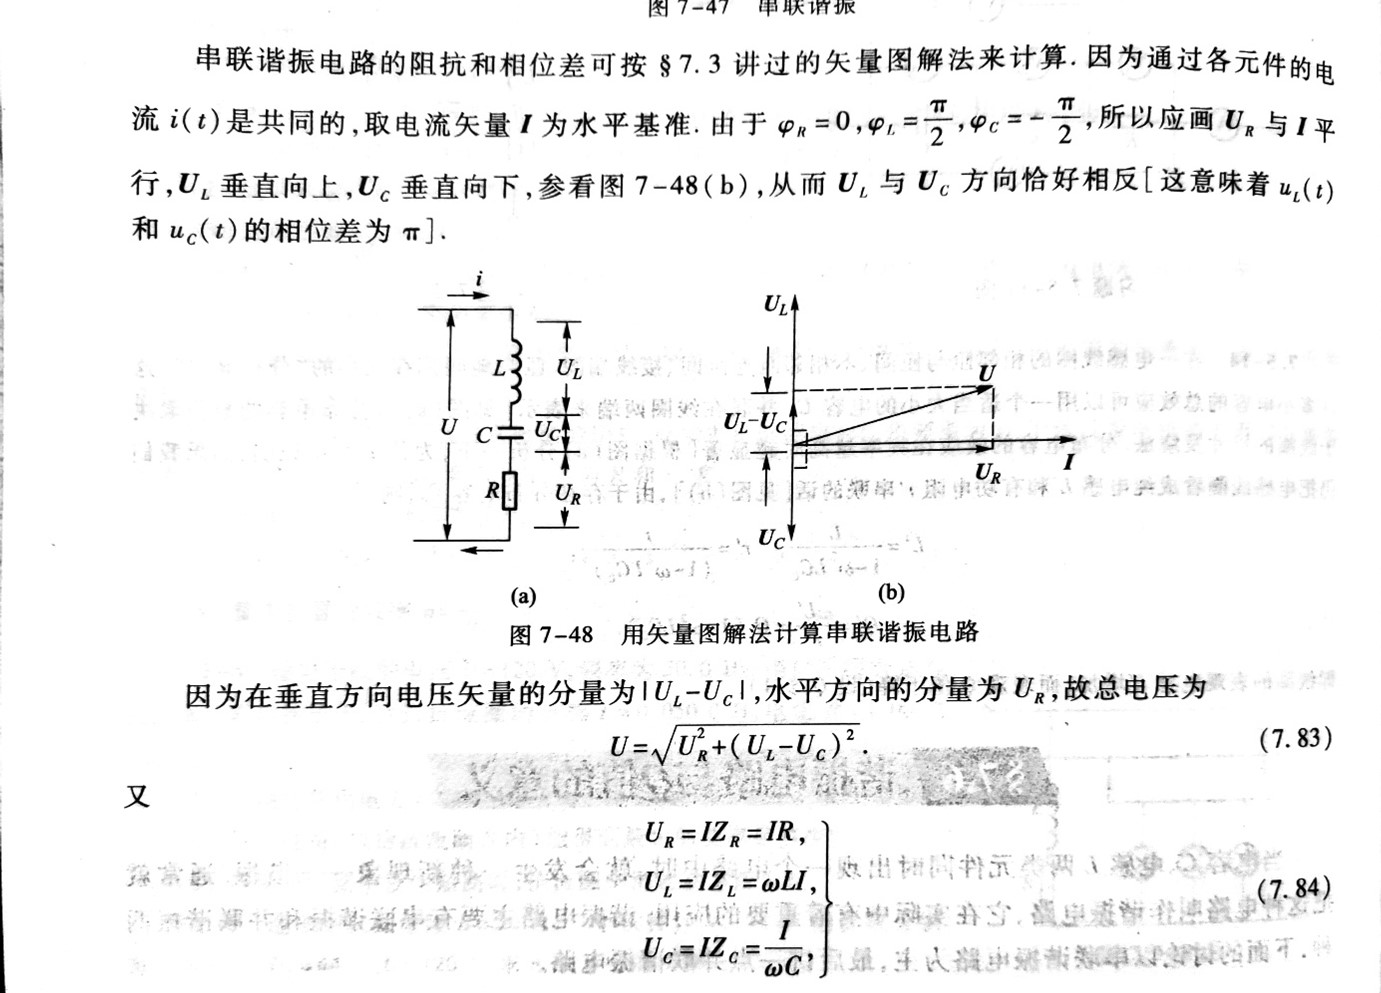
\includegraphics[width=12cm]{Fig/1.jpg}
        \caption{串联谐振电路(来源:赵凯华,陈熙谋:《电磁学(第四版)》,p414)}
    \end{figure}
    \hspace*{2em}如图,电阻,电容,电感的阻抗可用矢量图解法计算。结果为:
        \[U=I\sqrt{R^2+\left(\omega L-\frac{1}{\omega C}\right)^2},Z=\sqrt{R^2+\left(\omega L-\frac{1}{\omega C}\right)^2},I=\frac{U}{\sqrt{R^2+\left(\omega L-\frac{1}{\omega C}\right)^2}}\]
    \hspace*{2em}相位角
        \[\varphi=arctan{\frac{U_L-U_C}{U_R}}=arctan\frac{\omega L-\frac{1}{\omega C}}{R}\]
    \hspace*{2em} 由相位角$\varphi$的表达式知,RLC谐振电路的容性,感性,阻性由$U_L-U_C$决定。$U_L-U_C>0$时,等价于LR电路,电路呈电感性。$U_L-U_C<0$时,等价于CR电路,电路呈电容性。$U_L-U_C=0$时,阻抗最小,电流最大,处于串联谐振状态。此时,有$\omega=\omega_0=\frac{1}{\sqrt{LC}}$,频率$f_0=\frac{\omega_0}{2\pi}=\frac{1}{2\pi\sqrt{LC}}$称为谐振频率。
    \newline \hspace*{2em}在交流电一个周期里,电阻元件消耗能量$W_R=RI^2T$。谐振电路中储存的能量为
        \[W_S=\frac{1}{2}Li^2+\frac{1}{2}Cu^2=\frac{1}{2}I_0^2\left( Lcos^2\omega t+\frac{1}{\omega^2C}sin^2\omega t \right)\]
    \hspace*{2em} 当$\omega=\frac{1}{\sqrt{LC}}$时,有$W_S=\frac{1}{2}LI_0^2=LI^2$。定义品质因数$Q=2\pi\frac{W_s}{W_R}=\frac{P_{ \text{无功} }}{P_{ \text{有功} }}$,品质因数为无量纲参数。品质因数越大,储能效果越好,耗散越少。
    \newline \hspace*{2em} 人为规定,在谐振峰两边$I$的值等于最大值$I_M$的$\frac{1}{\sqrt2}\approx70\%$处频率之间的宽度为通频带宽度。此时
    \[Q=2\pi f_0\frac{L}{R},\delta f=\mp\frac{f_0}{2Q},\ \Delta f=2\delta f=\frac{f_0}{Q}\]
    \hspace*{2em} 这里给出了品质因数$Q$的另一个定义。$Q$与$\Delta f$成反比,$Q$越大,通频带宽度越窄,选择性越好。
    \newline \hspace*{2em} 同时谐振时有
    \[Q=\frac{U_C}{U}=\frac{U_L}{U}=\frac{Z_C}{Z}=\frac{Z_L}{Z}=\frac{1}{\omega_0CR}=\frac{\omega_0L}{R}=\frac{1}{R}\sqrt{\frac{L}{C}}\]
    \hspace*{2em} 这证明了品质因数越大,频率选择性越好。同时,要注意电感和电容上的电压为电源的Q倍,能放大电路中局部电压,易超过36V,易发生危险。因此,品质因数也能体现电压分配特性。
    \begin{figure}[H]
        \begin{minipage}[t]{0.3\linewidth}
            \centering
            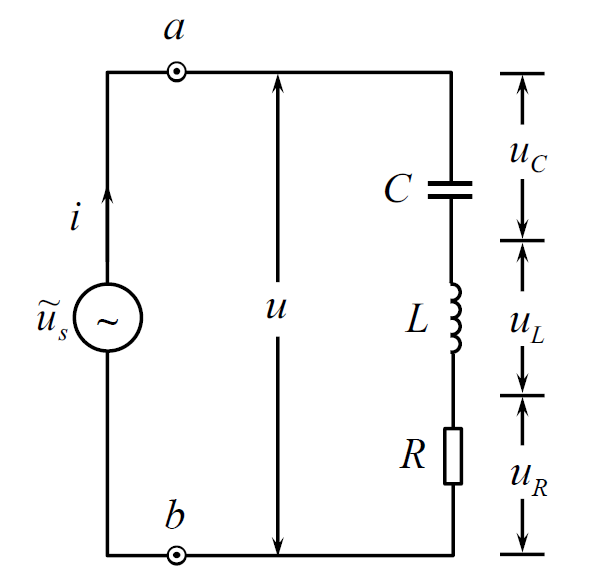
\includegraphics[width=4cm]{Fig/2.png}
            \caption{串联谐振电路}
        \end{minipage}
        \begin{minipage}[t]{0.69\linewidth}
            \centering
            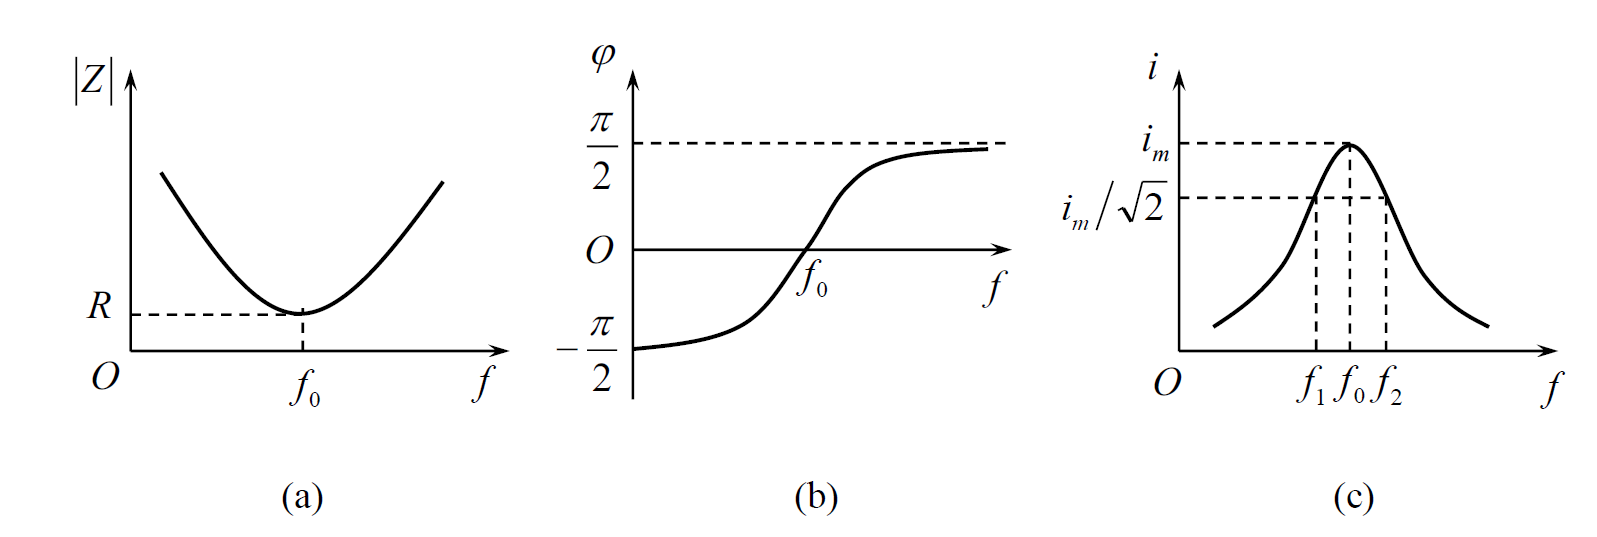
\includegraphics[width=11.5cm]{Fig/3.png}
            \caption{RLC串联电路的频率特性(a)阻抗特性;(b)相频特性;(c)幅频特性}
        \end{minipage}
    \end{figure}
    \item 并联谐振 \newline \hspace*{2em}
    相关阻抗,电压,幅角的计算方法与串联谐振电路相同。
    \[\text{阻抗}Z=\sqrt{\frac{R^2+\left(\omega L\right)^2}{\left(1-\omega^2LC\right)^2+\left(\omega CR\right)^2}}\]
    \[\text{幅角}\varphi=arctan\frac{\omega L-\omega C\left[R^2+\left(\omega L\right)^2\right]}{R}\]
    \[\text{谐振条件}f_0=\frac{\omega_0}{2\pi},f_p=\frac{\omega_p}{2\pi},\omega_0=\frac{1}{\sqrt{LC}},\omega_p=2\pi f_p=\sqrt{\frac{1}{LC}-\left(\frac{R}{L}\right)^2}=\omega_0\sqrt{1-\frac{1}{Q^2}}\]
    \hspace*{2em} $f_0$与$f_p$略有不同。当$Q>>1$时,两者相近。
    \begin{figure}[H]
        \begin{minipage}[t]{0.3\linewidth}
            \centering
            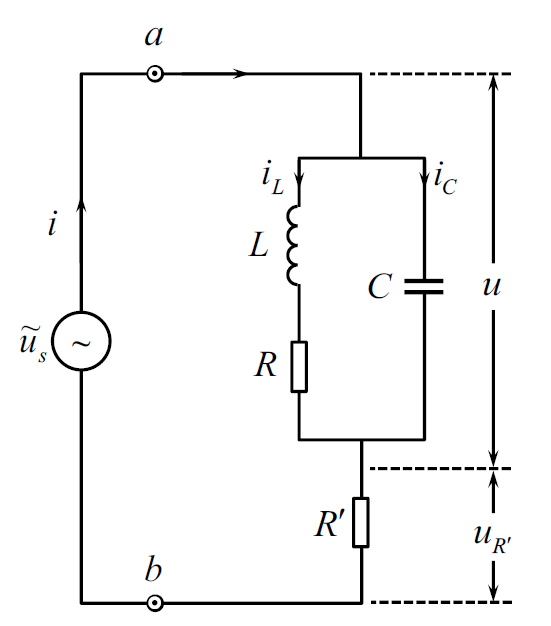
\includegraphics[width=4cm]{Fig/4.png}
            \caption{并联谐振电路}
        \end{minipage}
        \begin{minipage}[t]{0.69\linewidth}
            \centering
            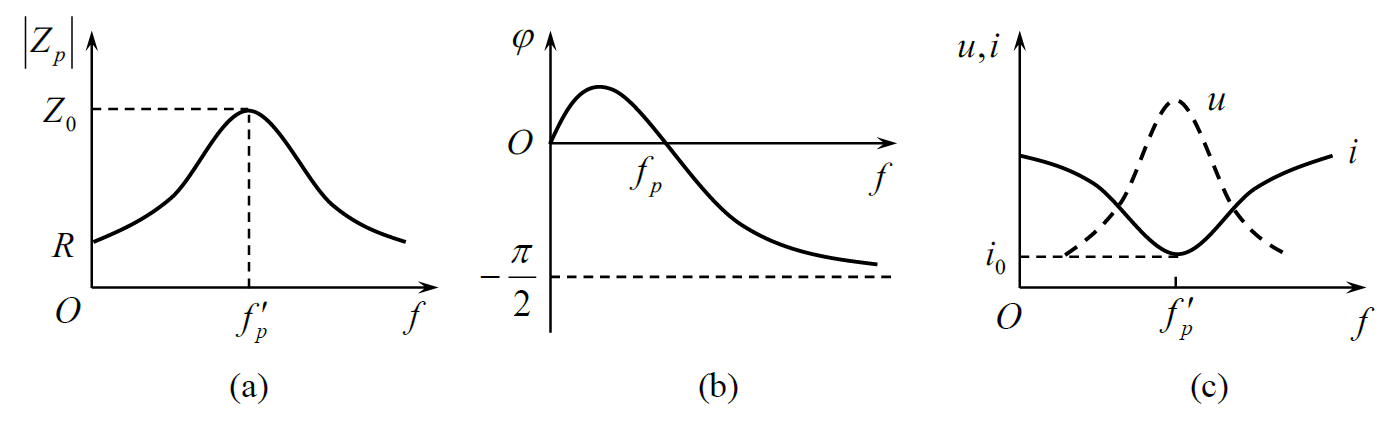
\includegraphics[width=11.5cm]{Fig/5.png}
            \caption{RLC 并联电路的频率特性(a)阻抗特性;(b)相频特性;(c)幅频特性}
        \end{minipage}
    \end{figure}
    \item RLC谐振电路暂态过程
    \newline \hspace*{2em}由电路的微分方程
    \[L\frac{di}{dt}+iR+\frac{q}{C}=\begin{cases}0,&\text{S接于1}\\ \epsilon,&\text{S接于2}\end{cases}\]
    \hspace*{2em} 其中$i=\frac{dq}{dt}=C\frac{du_c}{dt}$,带入后解微分方程得到一组解:
    \[
        q=\begin{cases}
        \left\{ \begin{matrix}{C\epsilon}\\0\\\end{matrix}\right\}\mp C\epsilon\frac{1}{\sqrt{1-\lambda^2}}e^{-\alpha t}\cos{\left(\sqrt{-\beta^2}-\arctan{\frac{\alpha}{\sqrt{-\beta^2}}}\right)}  &(0<\lambda<1 \text{,阻尼振荡;}\lambda=0 \text{,无阻尼振荡})\\
        \left\{ \begin{matrix}{C\epsilon}\\0\\\end{matrix}\right\}\mp C\epsilon e^{-\alpha t}\left( 1+\alpha t\right)  &(\lambda=1 \text{,临界阻尼})\\
        \left\{ \begin{matrix}{C\epsilon}\\0\\\end{matrix}\right\}\mp C\epsilon \frac{1}{2\beta} e^{-\alpha t}\left[ \left( \alpha + \beta\right)e^{\beta t}-\left( \alpha - \beta \right)e^{-\beta t}  \right] &(\lambda>1 \text{,过阻尼})
        \end{cases}
    \]
    \hspace*{2em}其中
    \[
        \text{阻尼系数}\lambda=\frac{R}{2} \sqrt{\frac{C}{L}},\quad
        \alpha=\frac{R}{2L},\quad
        \beta^2=\alpha^2-\frac{1}{LC}=\frac{\lambda^2-1}{LC}
    \]
    \hspace*{2em}可以看出,阻尼振荡时周期(频率)不变。充电和放电q-t曲线仅有初相位的区别。
    \begin{figure}[H]
        \begin{minipage}[t]{0.33\linewidth}
            \centering
            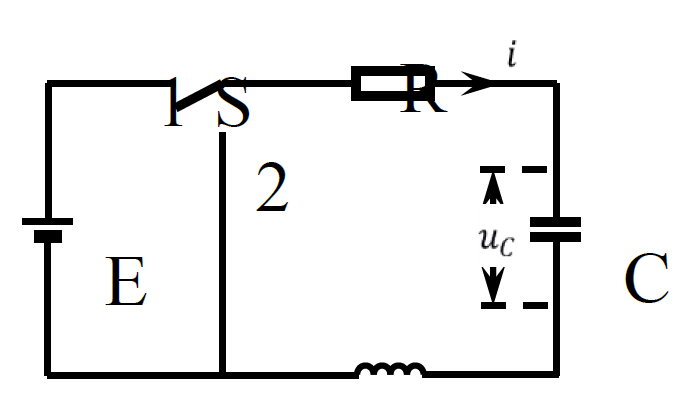
\includegraphics[width=5.5cm]{Fig/7.png}
            \caption{RLC电路暂态过程}
        \end{minipage}
        \begin{minipage}[t]{0.33\linewidth}
            \centering
            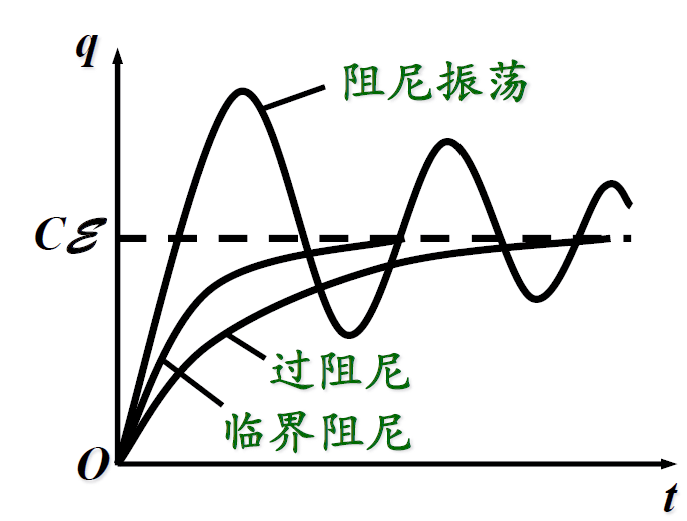
\includegraphics[width=5.5cm]{Fig/6-充电.png}
            \caption{充电时q-t曲线}
        \end{minipage}
        \begin{minipage}[t]{0.33\linewidth}
            \centering
            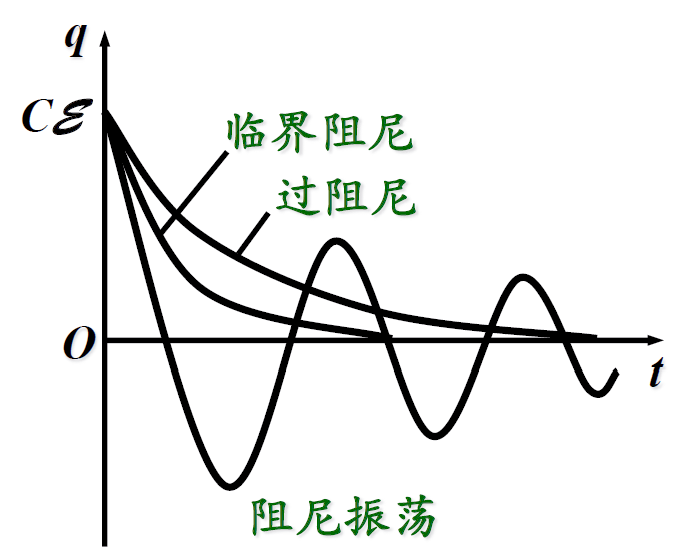
\includegraphics[width=5.5cm]{Fig/6-放电.png}
            \caption{放电时q-t曲线}
        \end{minipage}
    \end{figure}
\end{enumerate}


\section{实验内容}
    
\subsection {RLC 串联电路的相频特性和幅频特性曲线}

\begin{enumerate}
    \item 实验步骤
    \begin{enumerate}
        \item 如图2,连接串联谐振电路。信号发生器充当电源(注意红端不要直接接在电阻旁)。将示波器CH1接在整个电路测总电压$U$,CH2接在电阻两端测电阻两端的电压$U_R$。
        \item 调整信号发生器输出电压为2V$(V_{pp})$。调整信号发生器输出频率,测$U$与$U_R$的相位差$\varphi$,测$U_R$的幅度值,记录数据。
        \item 改变信号发生器输出频率,重复b),进行多组实验,记录数据。
    \end{enumerate}
    \item 实验数据
    \[\text{电阻}R=100\Omega \quad \text{电容}C=0.05\mu F \quad \text{电感}L=0.1H \]
    \[\text{由此计算出}f_0=\frac{1}{2\pi\sqrt{LC}}=2250.79Hz,Q=\frac{1}{R}\sqrt{\frac{L}{C}}=14.1\]
    \hspace*{2em} 本次试验中,直接使用示波器相位差模式测量相位差$\varphi$。测量时探头倍数为$\times 10$,因此下表数据为测量数据的十分之一。测量数据中最后一组测量值为负数,实际应为正数,进行修正。
    \newline \hspace*{2em}测量时,使用Avg,等待一段时间后读取平均值,平均值较为稳定。测量完一组数据后关闭Avg模式再打开,刷新数据。
    \newline \hspace*{2em}表中,测量值为$U,\varphi,U_{R}$;幅值为最大值的两倍,$I_{max}=\frac{U_{Rmax}}{R}=\frac{U_R}{2R}$为理论计算值,。
    \newline \hspace*{2em}下图中,得出结果与图3(b)(c)相符。本串联谐振电路的谐振频率约为$f_0=2.25kHz$。
    \newline \hspace*{2em}在$2V$输入电压下,万用表测量值$U_L=U_C=5.18V$,注意万用表测量的是有效值,示波器测量的是幅值,幅值是有效值的$2\sqrt{2}$倍。品质因数约为$Q=\frac{U_L}{U}=\frac{U_C}{U}=7.33$,与理论值相差很大。数据表上测量的$U$偏差更大,可忽略。
    % Table generated by Excel2LaTeX from sheet 'Sheet1'
        \begin{table}[H]
          \centering
          \caption{串联谐振的相频特性和幅频特性}
            \begin{tabular}{|r|r|r|r|r|}\hline
            $f/kHz$ &$U(V_{pp})/V$  &$\left(CH1-CH2\right)\varphi/^\circ$  &$U_{R} \left(V_{amp}\right) /V$  &$I_{max}/mA$\\\hline

            1.88   & 2.00   & -81    & 0.314  & 1.57 \\\hline
            2      & 2.00   & -73    & 0.490  & 2.45 \\\hline
            2.08   & 2.00   & -63    & 0.704  & 3.52 \\\hline
            2.15   & 2.00   & -47    & 0.800  & 4 \\\hline
            2.19   & 2.00   & -33    & 0.930  & 4.65 \\\hline
            2.22   & 2.00   & -18    & 0.983  & 4.915 \\\hline
            2.24   & 2.00   & -7     & 0.997  & 4.985 \\\hline
            2.25   & 2.00   & -1.2   & 1.000  & 5 \\\hline
            2.26   & 2.00   & 5.5    & 0.991  & 4.955 \\\hline
            2.275  & 2.00   & 12     & 0.991  & 4.955 \\\hline
            2.3    & 2.00   & 25     & 0.963  & 4.815 \\\hline
            2.36   & 2.00   & 47     & 0.778  & 3.89 \\\hline
            2.43   & 2.00   & 57     & 0.590  & 2.95 \\\hline
            2.62   & 2.00   & 66     & 0.366  & 1.83 \\\hline
            3.18   & 2.00   & 77     & 0.193  & 0.965 \\\hline

            \end{tabular}%
          \label{tab:串联谐振}%
        \end{table}%
        \begin{figure}[H]
            \begin{minipage}[t]{0.47\linewidth}
                \centering
                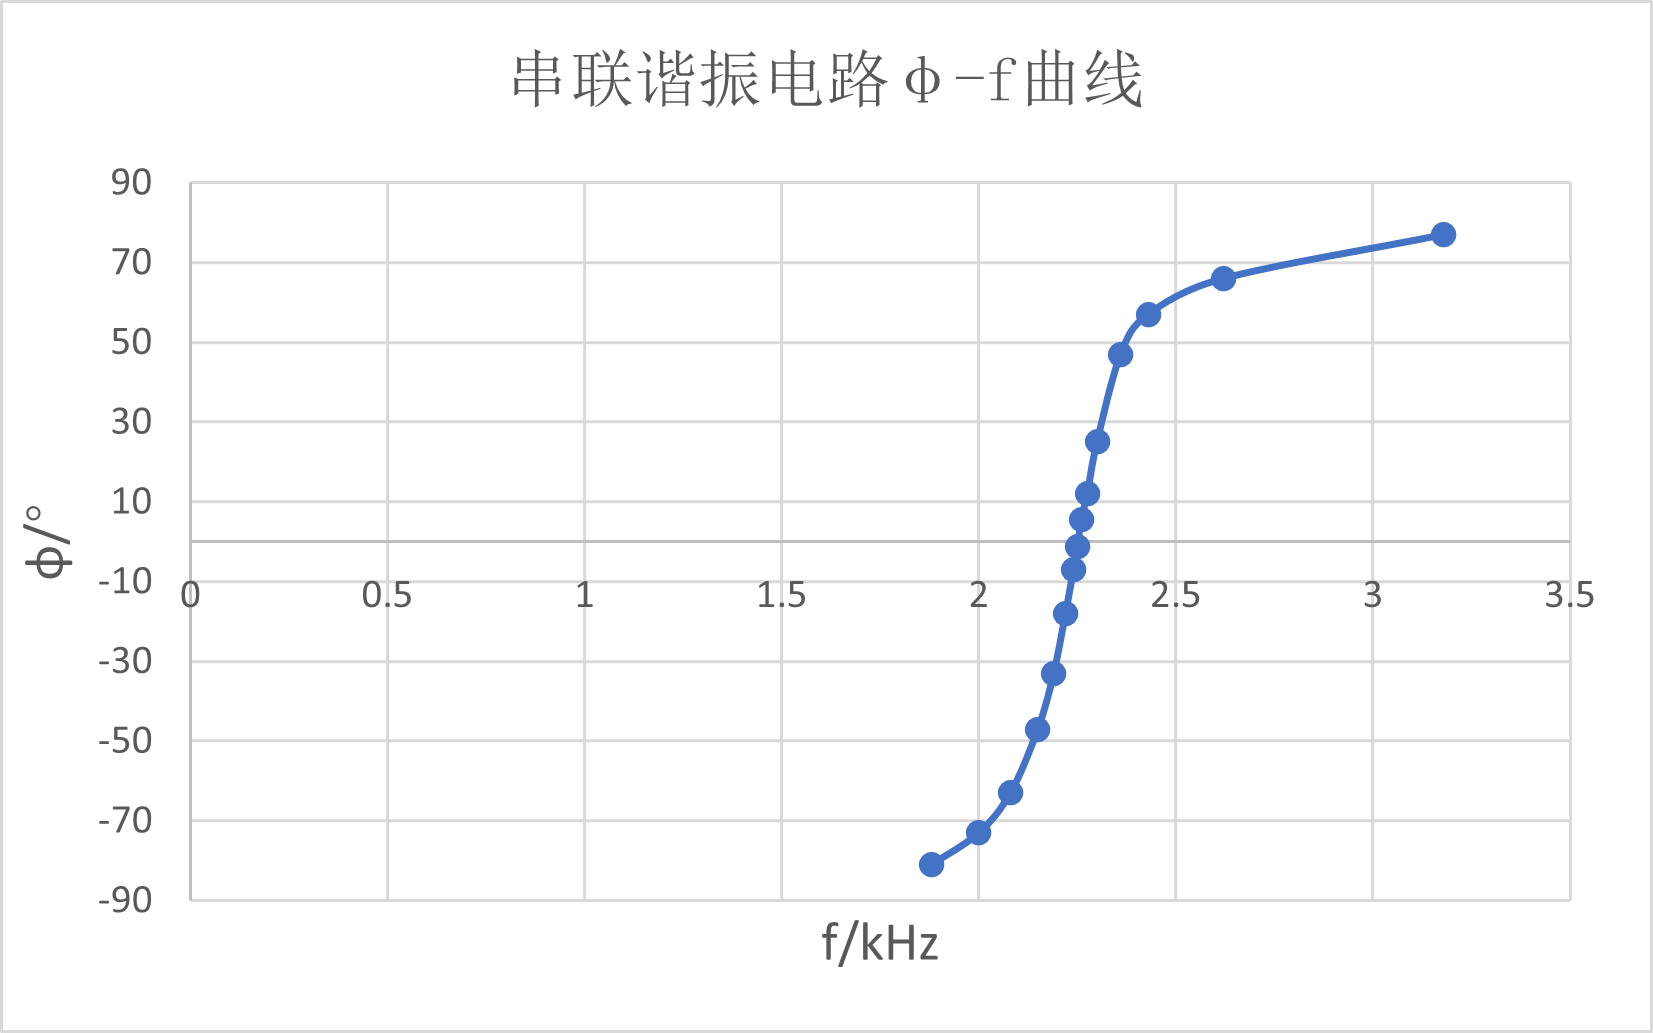
\includegraphics[width=7.5cm]{Fig/8-φf.png}
                \caption{串联谐振电路$\varphi - f$曲线}
            \end{minipage}
            \begin{minipage}[t]{0.52\linewidth}
                \centering
                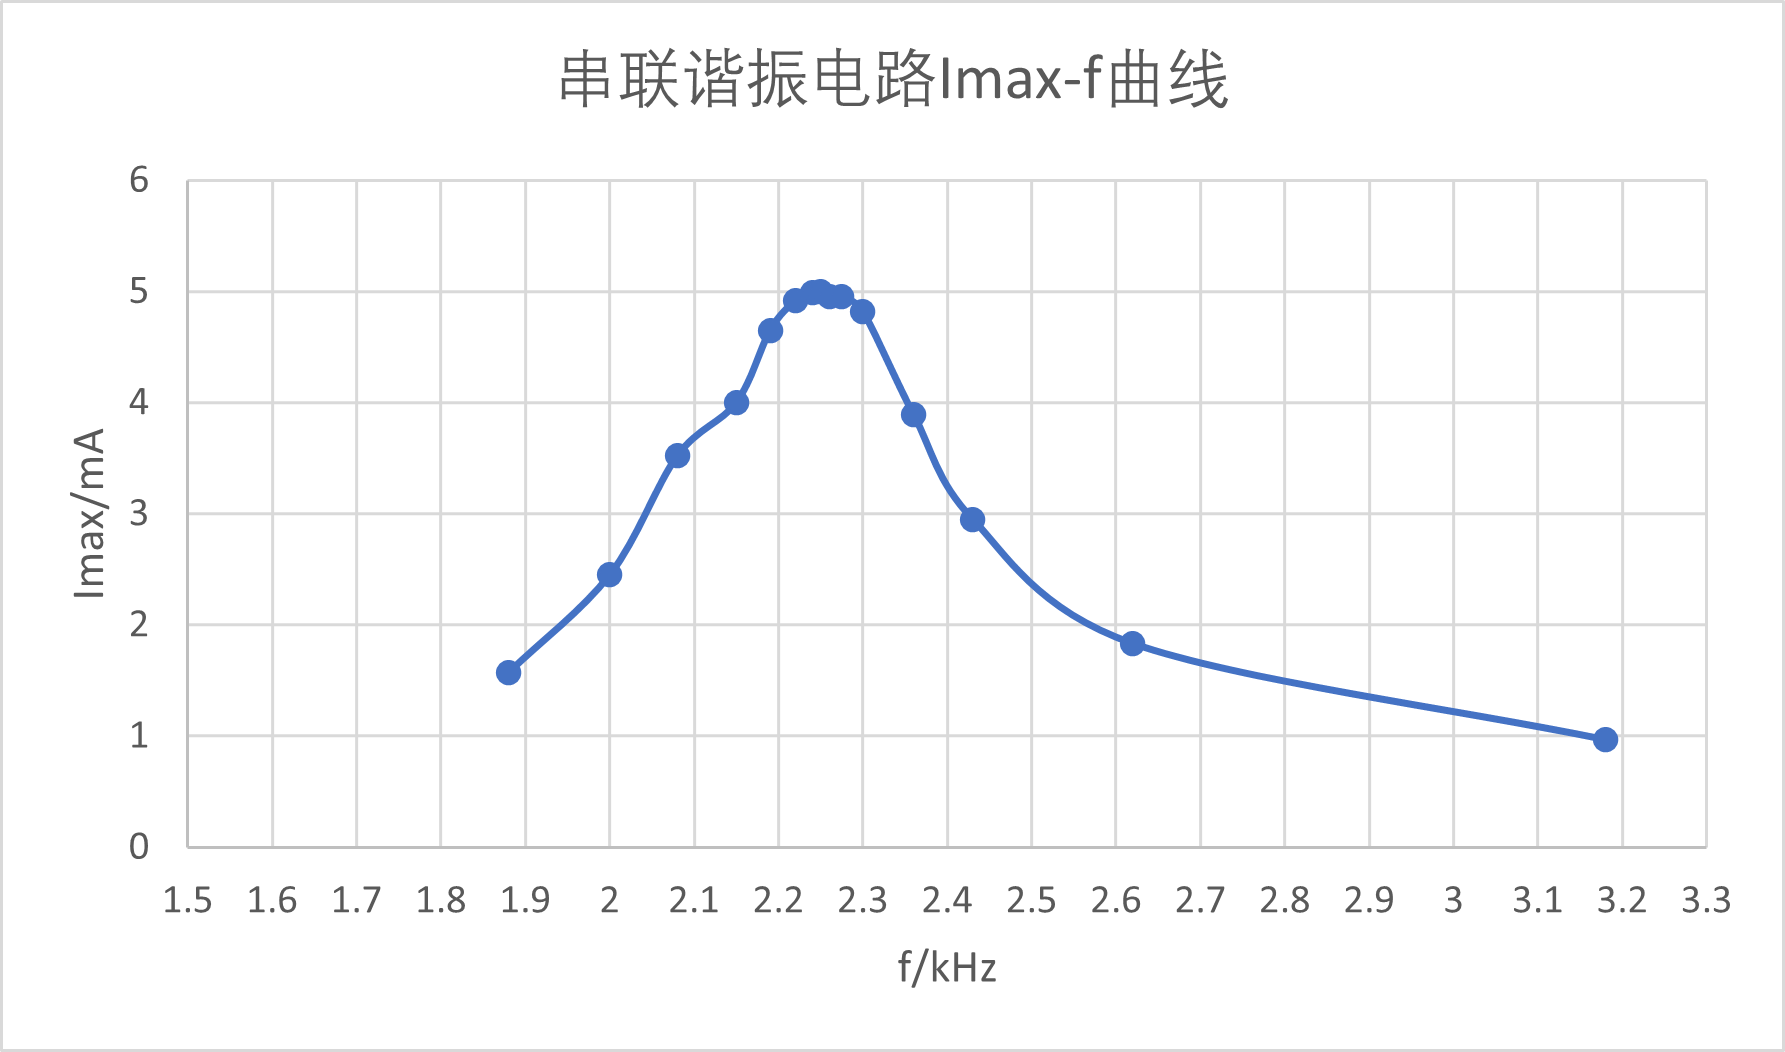
\includegraphics[width=8.5cm]{Fig/8-if.png}
                \caption{串联谐振电路$I_{max} - f$曲线}
            \end{minipage}
        \end{figure}
    由图10,通频带宽度$\Delta f \approx 2.38-2.08=0.3kHz \quad Q=\frac{f_0}{\Delta f}=7.5$,与理论值相差约为2倍。
    \item 实验总结
    \begin{enumerate}
        \item 本次实验中,测量数据与理论值相差较大。主要原因是:示波器未调整良好,探头倍数未设置为$\times 1$,导致测量误差较大。本实验中,电压不超过10V,为低电压,用$\times 1$精度更高,信号衰减导致严重误差。次要原因可能是接线不牢固、导线老化等原因导致的信号输出不稳定,致使读数偏差。实验中,确实存在静置设备一段时间长时间输出后结果不相近,特别是电压。
        \item 本实验中的相位差测量较为准确,最后一组读取时出现负值,出现异常,理论上应为正值。可能是测量时相位差不是严格的(CH1-CH2),可能变动为了(CH2-CH1)。对相位差的正负应人工修正。
        \item 在已接好RLC的情况下,信号发生器输出正极接在电阻边不产生谐振现象,而接在电容/电感边产生谐振现象。原因是:信号发生器正极产生正弦波形,负极为0V,如此产生交流电。若正极先接在电阻旁,电压经过衰减后才进入电容和电感,会使谐振现象不明显乃至无法观察。
    \end{enumerate}
   
\end{enumerate}
\subsection{RLC 并联电路的相频特性和幅频特性曲线}
\begin{enumerate}
    \item 实验步骤
    \begin{enumerate}
        \item 如图4,连接并联谐振电路。信号发生器充当电源(注意红端不要直接接在电阻旁)。将示波器CH1接在整个电路测总电压$U_0$,CH2接在电阻两端测电阻两端的电压$U_R$。用示波器math功能计算$U=U_0-U_R$的波形。
        \item 调整信号发生器输出电压为2V$(V_{pp})$。调整信号发生器输出频率,测$U$与$U_R$的时间差$\Delta t$,从而计算$\varphi=f\Delta t\times 360^\circ$。测$U_R$的幅度值,记录数据。
        \item 改变信号发生器输出频率,重复b),进行多组实验,记录数据。
    \end{enumerate}
    \item 实验数据
    \[\text{电阻}R'=5k\Omega \quad \text{电容}C=0.05\mu F \quad \text{电感}L=0.1H \]
    \[\text{由此计算出}f_0=\frac{1}{2\pi\sqrt{LC}}=2250.79Hz,Q=\frac{1}{R'}\sqrt{\frac{L}{C}}=0.28\]
    \hspace*{2em} 本次试验中,使用测量峰值时间差$\Delta t$的方式计算相位差$\varphi$。测量时探头倍数为$\times 10$,因此下表电压数据为测量数据的十分之一。
    \newline \hspace*{2em}测量时,应使用Avg,等待一段时间后读取平均值,平均值较为稳定。测量完一组数据后关闭Avg模式再打开,刷新数据。但测量时间差时,我忘记打开Avg模式了,直接读取瞬间值,导致数据不稳定,会产生一定误差。


            % Table generated by Excel2LaTeX from sheet 'Sheet1'
        \begin{table}[htbp]
          \centering
          \caption{并联电路的相频特性和幅频特性}
            \begin{tabular}{|r|r|r|r|r|r|r|}\hline
            $f/kHz$ & $U_0(V_{pp})/V$ & $\Delta t/ms$ & $\varphi /\circ$ & $U(V_{amp})/V(CH1-CH2)$ & $U_R(V_{amp})/mV(CH2)$ & $I_{max}/mA$ \\\hline
            
            2.050  & 2.00   & -105   & 77.5   & 1.62   & 1070   & 0.107 \\\hline
            2.150  & 2.00   & -100   & 73.4   & 1.78   & 597    & 0.0597 \\\hline
            2.200  & 2.00   & -88    & 69.7   & 1.84   & 332    & 0.0332 \\\hline
            2.231  & 2.00   & -63.6  & 51.5   & 1.86   & 174    & 0.0174 \\\hline
            2.240  & 2.00   & -50    & 40.32  & 1.85   & 136    & 0.0136 \\\hline
            2.247  & 2.00   & -21.2  & 17.1   & 1.85   & 118    & 0.0118 \\\hline
            2.250  & 2.00   & -8.8   & 7.1    & 1.85   & 114    & 0.0114 \\\hline
            2.253  & 2.00   & 1.1    & -0.9   & 1.86   & 113    & 0.0113 \\\hline
            2.256  & 2.00   & 9.2    & -7.5   & 1.86   & 114    & 0.0114 \\\hline
            2.265  & 2.00   & 40.4   & -32.9  & 1.86   & 135    & 0.0135 \\\hline
            2.275  & 2.00   & 60.4   & -49.5  & 1.86   & 175    & 0.0175 \\\hline
            2.320  & 2.00   & 87     & -72.7  & 1.83   & 396    & 0.0396 \\\hline
            2.400  & 2.00   & 88     & -76    & 1.71   & 787    & 0.0787 \\\hline
            2.600  & 2.00   & 91     & -85.2  & 1.34   & 1380   & 0.138 \\\hline

            \end{tabular}%
          \label{tab:并联电路的相频特性和幅频特性}%
        \end{table}%
        \begin{figure}[H]
            \begin{minipage}[t]{0.33\linewidth}
                \centering
                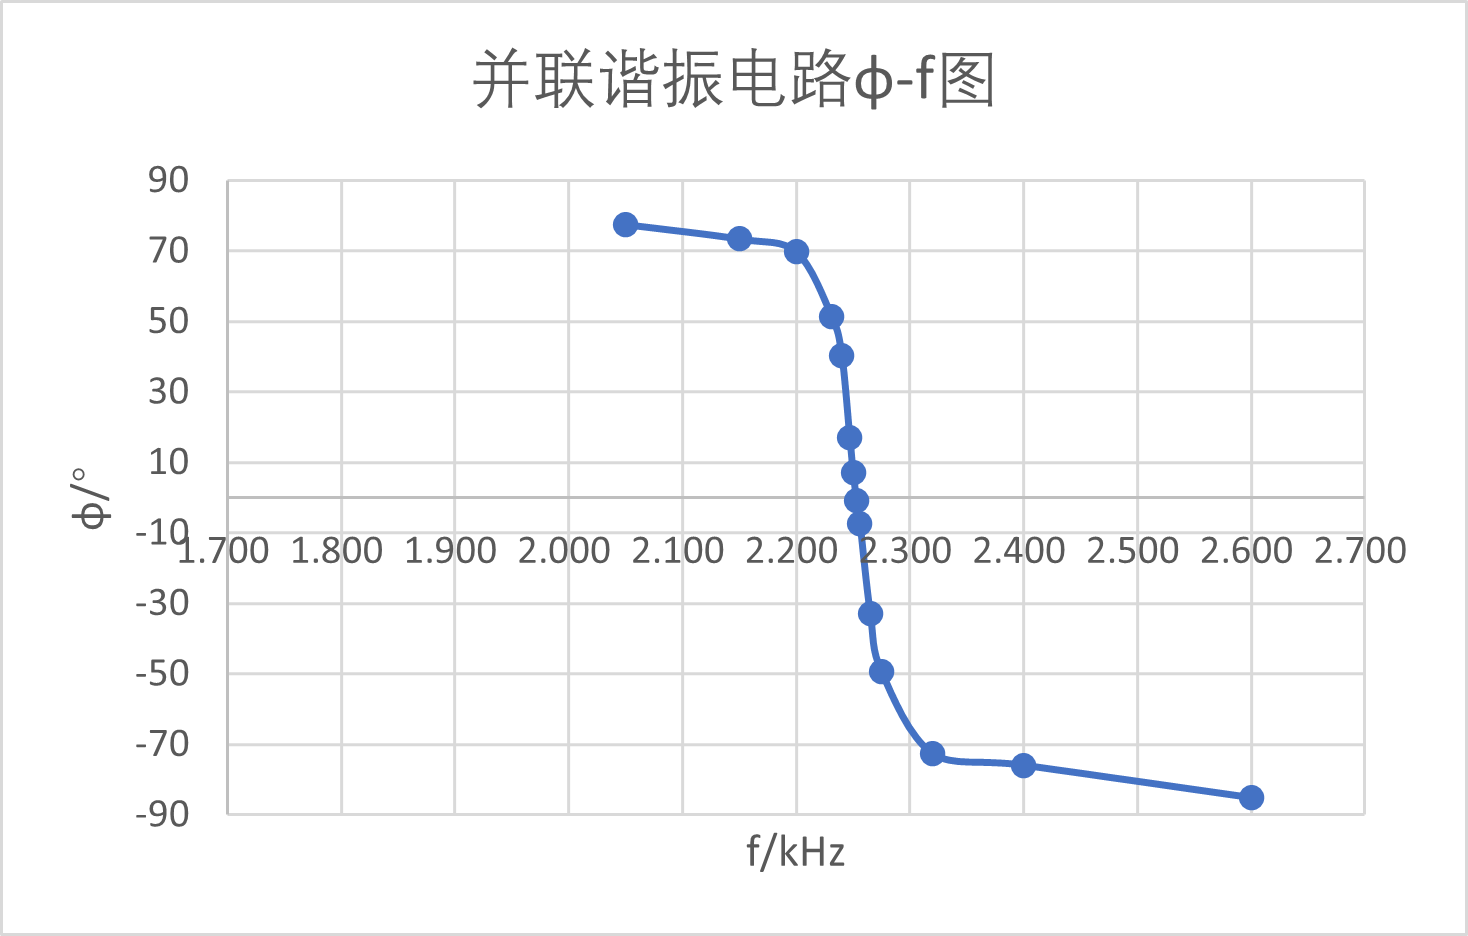
\includegraphics[width=5.5cm]{Fig/9-φf.png}
                \caption{并联谐振电路$\varphi - f$曲线}
            \end{minipage}
            \begin{minipage}[t]{0.33\linewidth}
                \centering
                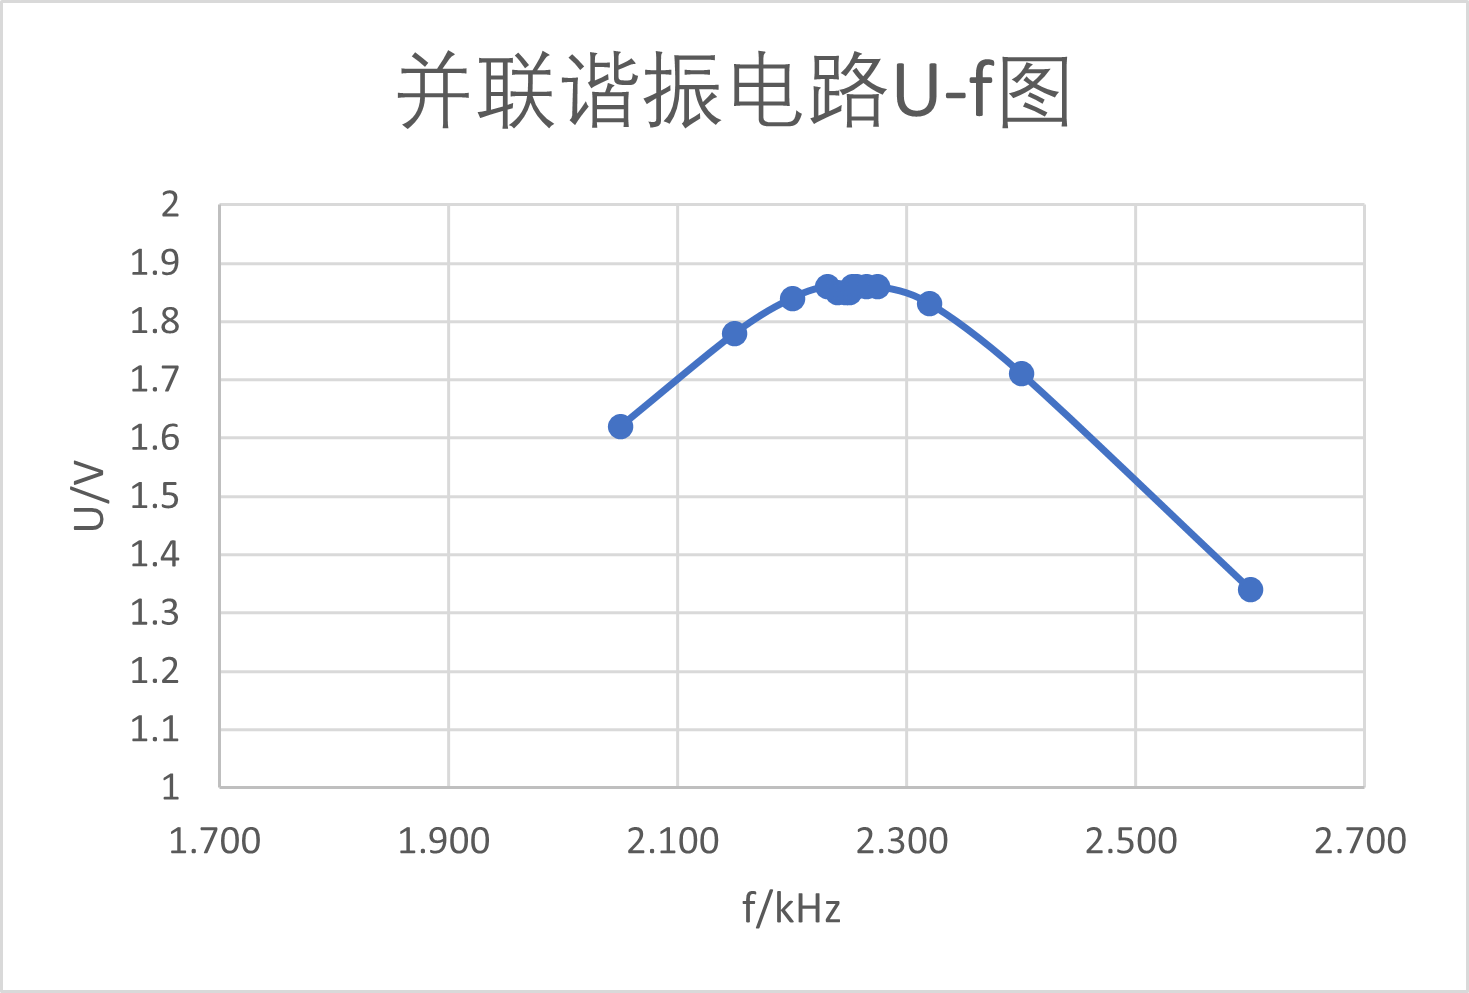
\includegraphics[width=5.5cm]{Fig/9-uf.png}
                \caption{并联谐振电路$U - f$曲线}
            \end{minipage}
            \begin{minipage}[t]{0.33\linewidth}
                \centering
                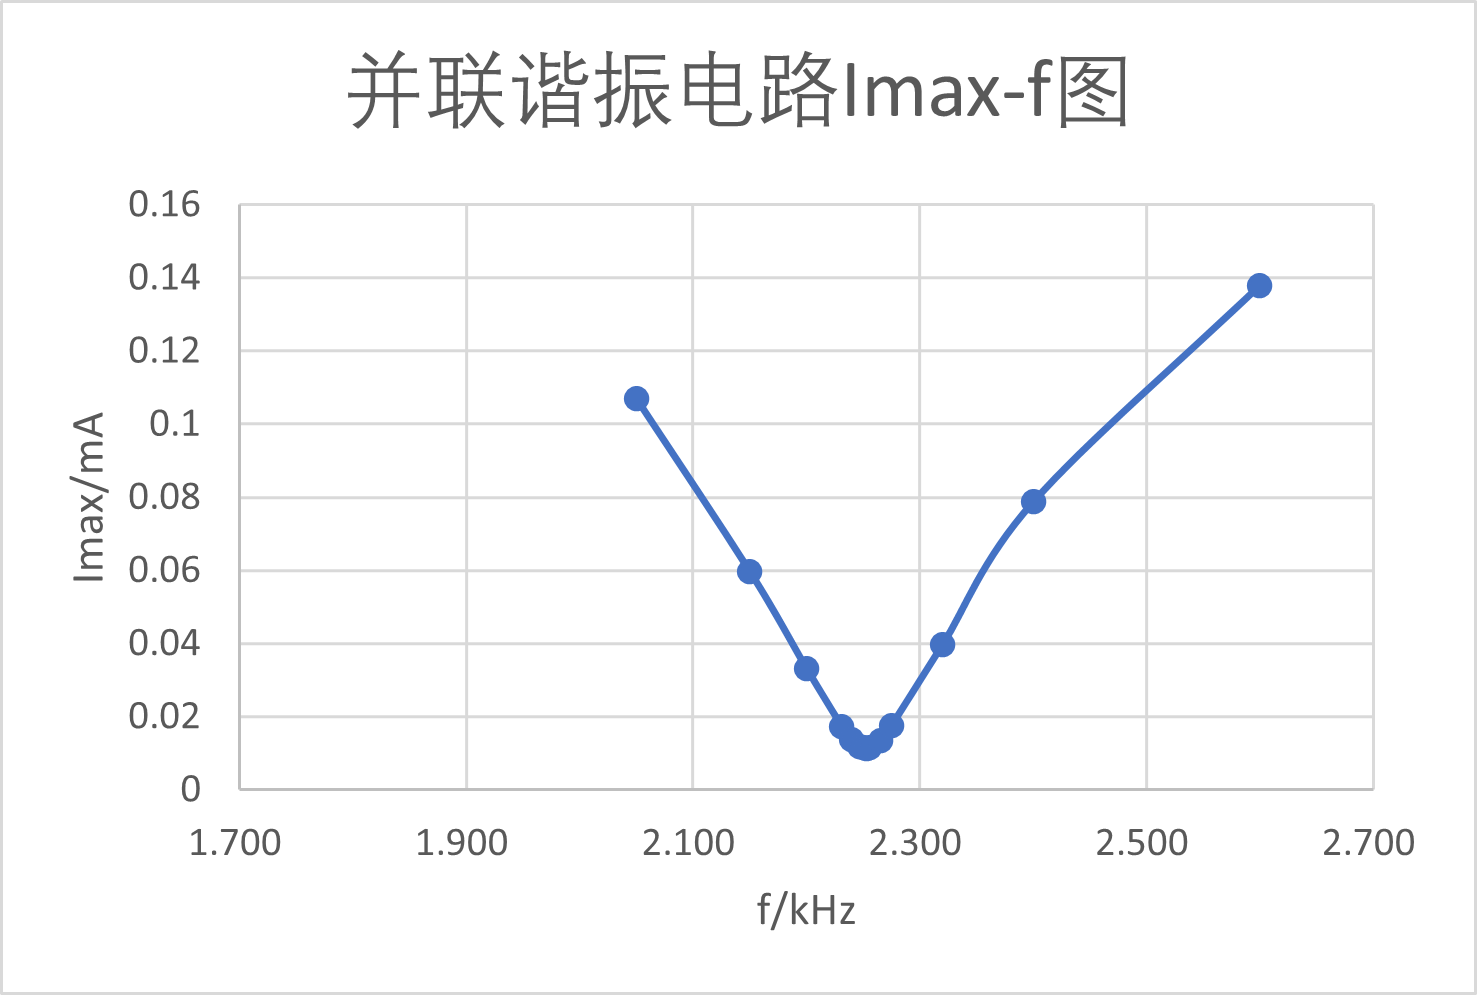
\includegraphics[width=5.5cm]{Fig/9-if.png}
                \caption{并联谐振电路$I_{max} - f$曲线}
            \end{minipage}
        \end{figure}
        \hspace*{2em}和图5的图像相近。本并联谐振电路的谐振频率约为$f_0=2.253kHz$,$f_0$和$f_p$相近。$\varphi\text{-}i$图像缺失频率较低的部分数据,无法判断低频时图像。
        \newline \hspace*{2em}数据上,对$\Delta t$和$\varphi$相对于测量值取负数,进行修正。由$\varphi$的表达式,$\omega$极大时,相位角应为$-\frac{\pi}{2}$。、
        \item 实验总结
        \begin{enumerate}
            \item 在预习过后,应该能知道串联电路和并联电路$\varphi\text{-}i$图像的巨大不同,可以自行加入几组较低频率的数据补全$\varphi\text{-}i$图像。
            \item 本次实验未使用Avg功能,但是图像上来看误差尚可。同时,本次实验没有采用手动移动光标,而是用示波器的时间差功能,误差不会增加很大。
        \end{enumerate}
\end{enumerate}
\subsection{观测RLC串联电路的暂态过程}
\begin{enumerate}
    \item 实验步骤
    \begin{enumerate}
        \item 如图6,连接串联谐振电路。信号发生器充当电源(注意红端不要直接接在电阻旁)。调整信号发生器,输出最低电压0V,最高电圧2V,频率50Hz,偏移1V,输出方波,实现周期性暂态过程。
        \item 示波器CH1通道用来测量总电压,CH2用来测量电容两端电压$U_C$,注意两个通道必须共地(示波器内部共地)。
        \item 观察波形并记录。
        \item 分别改变电阻箱阻值,信号发生器频率,观察波形并记录。
    \end{enumerate}
    \item 实验数据
    \begin{enumerate}
        \item 第一组:$R=0\Omega,L=0.1H,C=0.2\mu F$
        \begin{figure}[H]
            \centering
            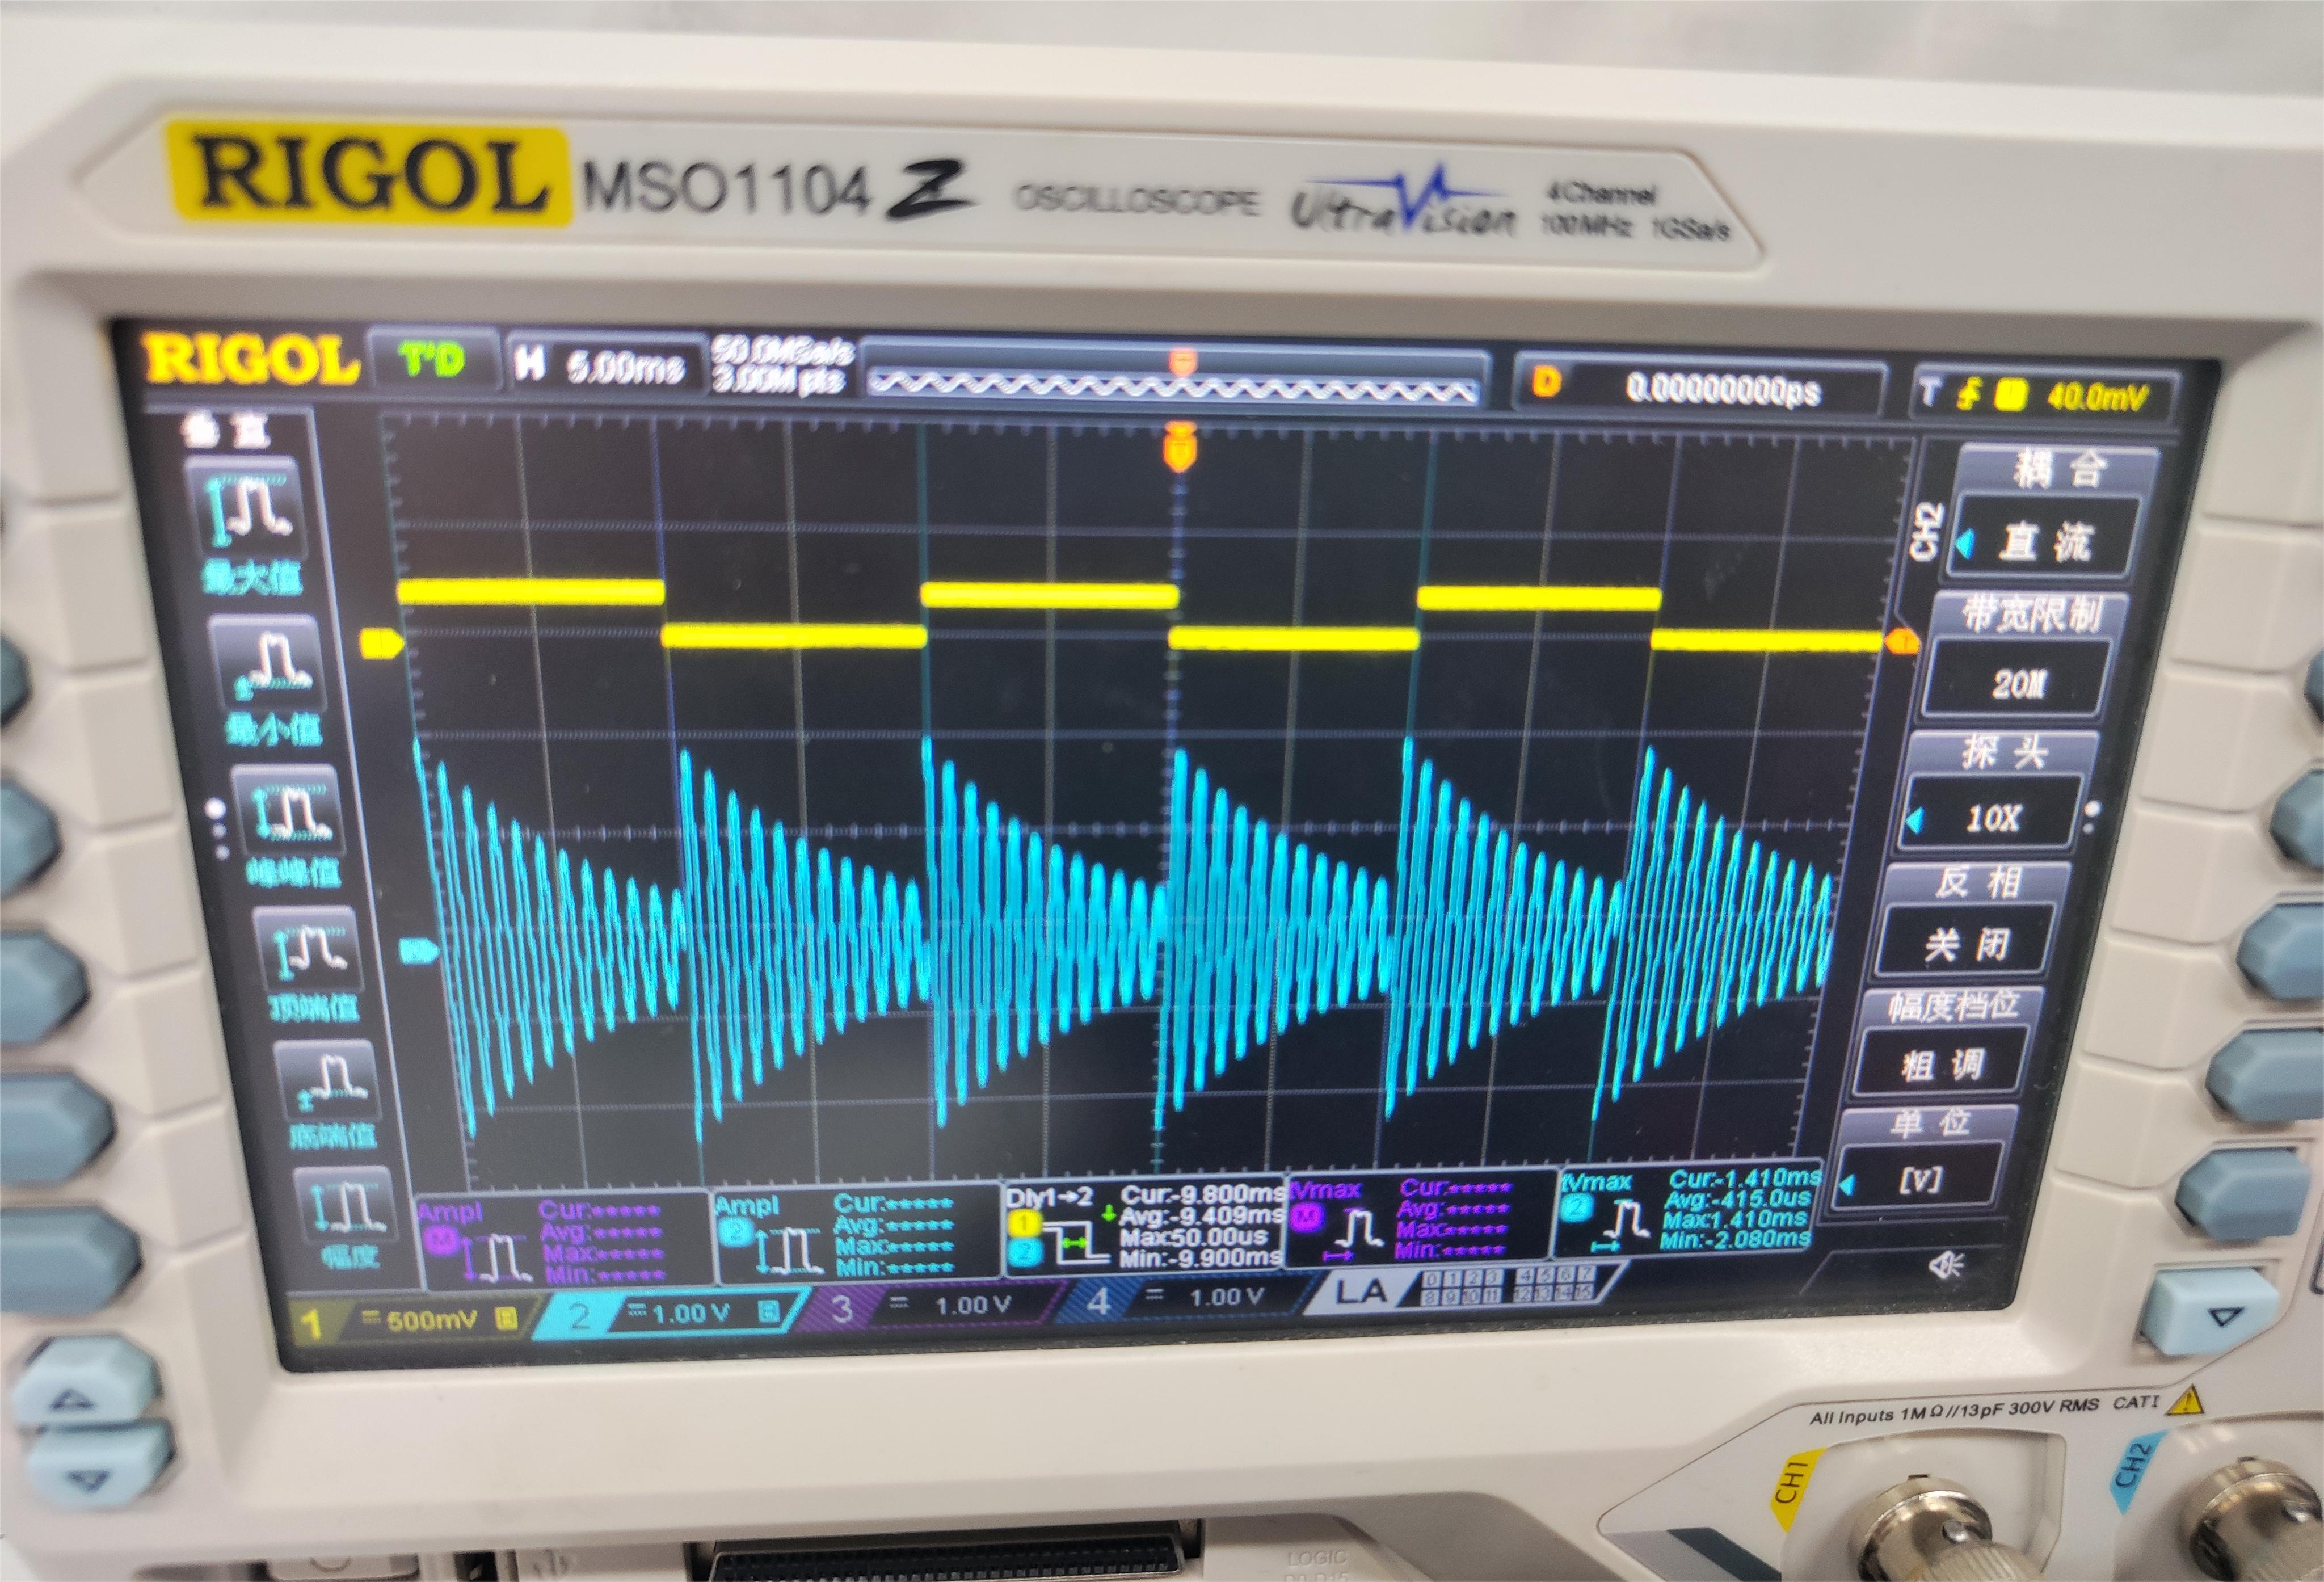
\includegraphics[width=10cm]{Fig/10.jpg}
            \caption{R=0$\Omega$时暂态过程}   
        \end{figure}
        \item 第二组:寻找临界电阻$R_c$,$L=0.1H,C=0.2\mu F$
        \begin{figure}[H]
            \begin{minipage}[t]{0.33\linewidth}
                \centering
                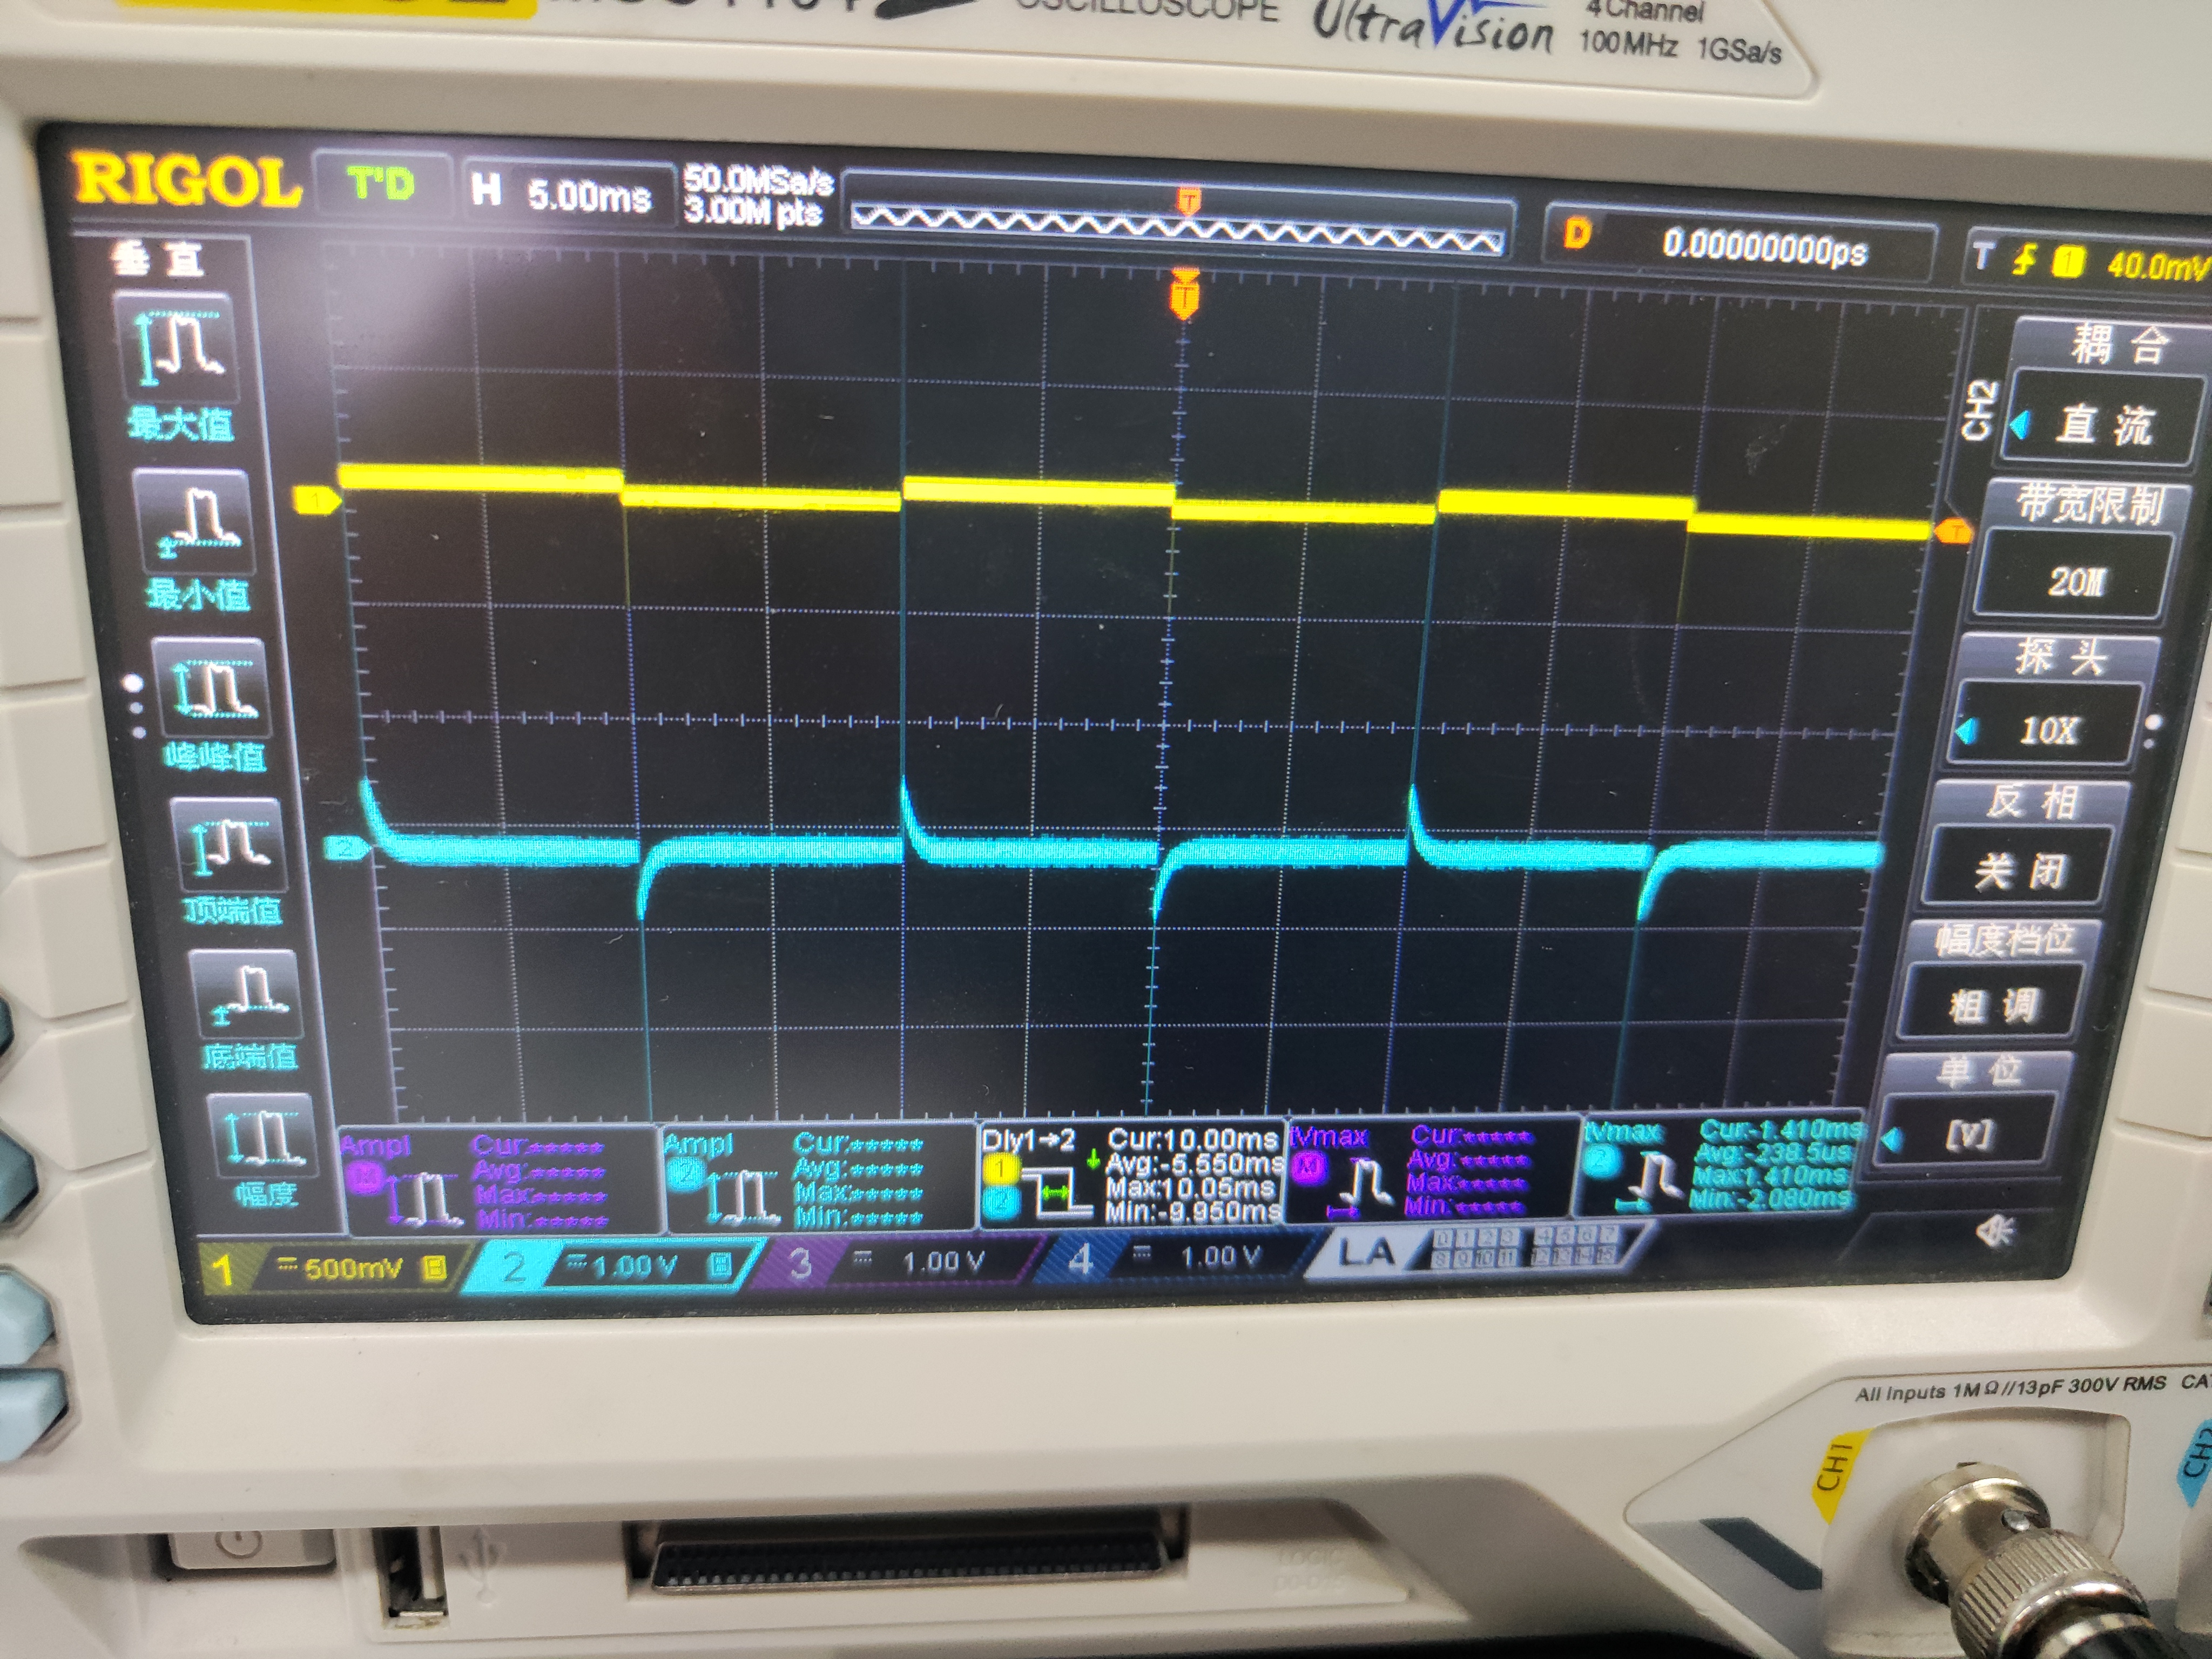
\includegraphics[width=5.5cm]{Fig/11.jpg}
                \caption{R=300$\Omega$时暂态过程}
            \end{minipage}
            \begin{minipage}[t]{0.33\linewidth}
                \centering
                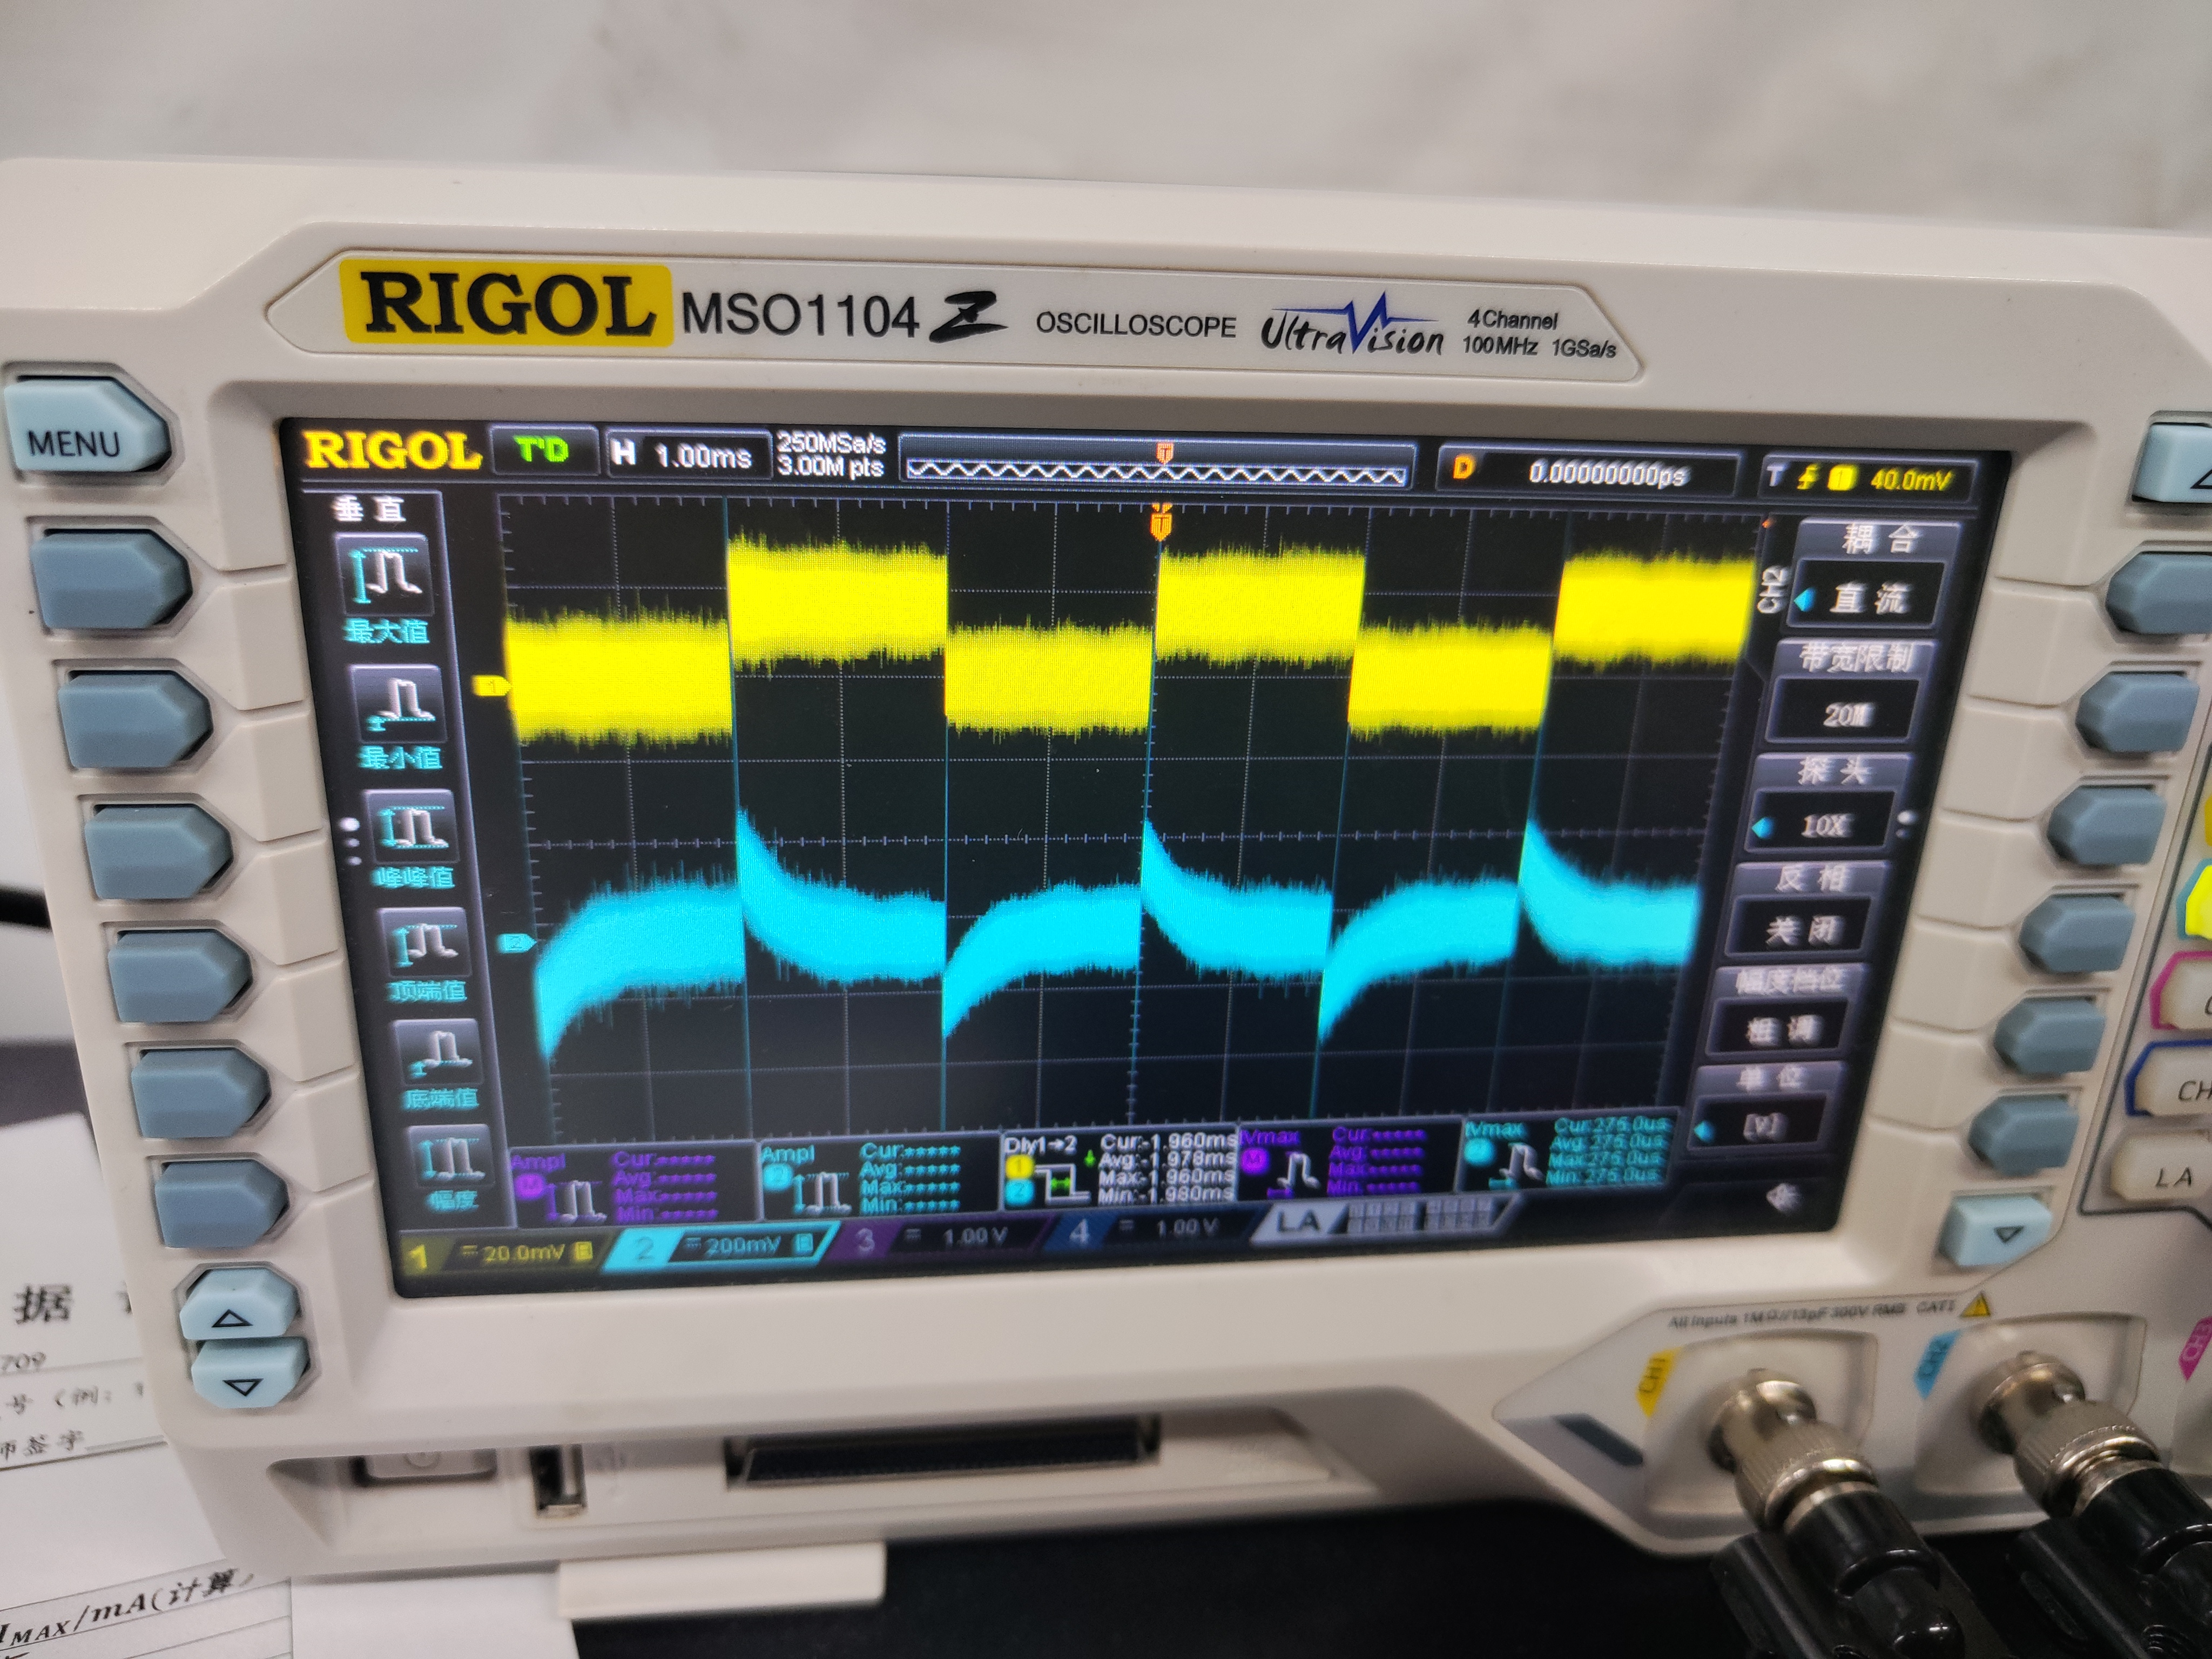
\includegraphics[width=5.5cm]{Fig/12.jpg}
                \caption{R=1300$\Omega$时暂态过程}
            \end{minipage}
            \begin{minipage}[t]{0.33\linewidth}
                \centering
                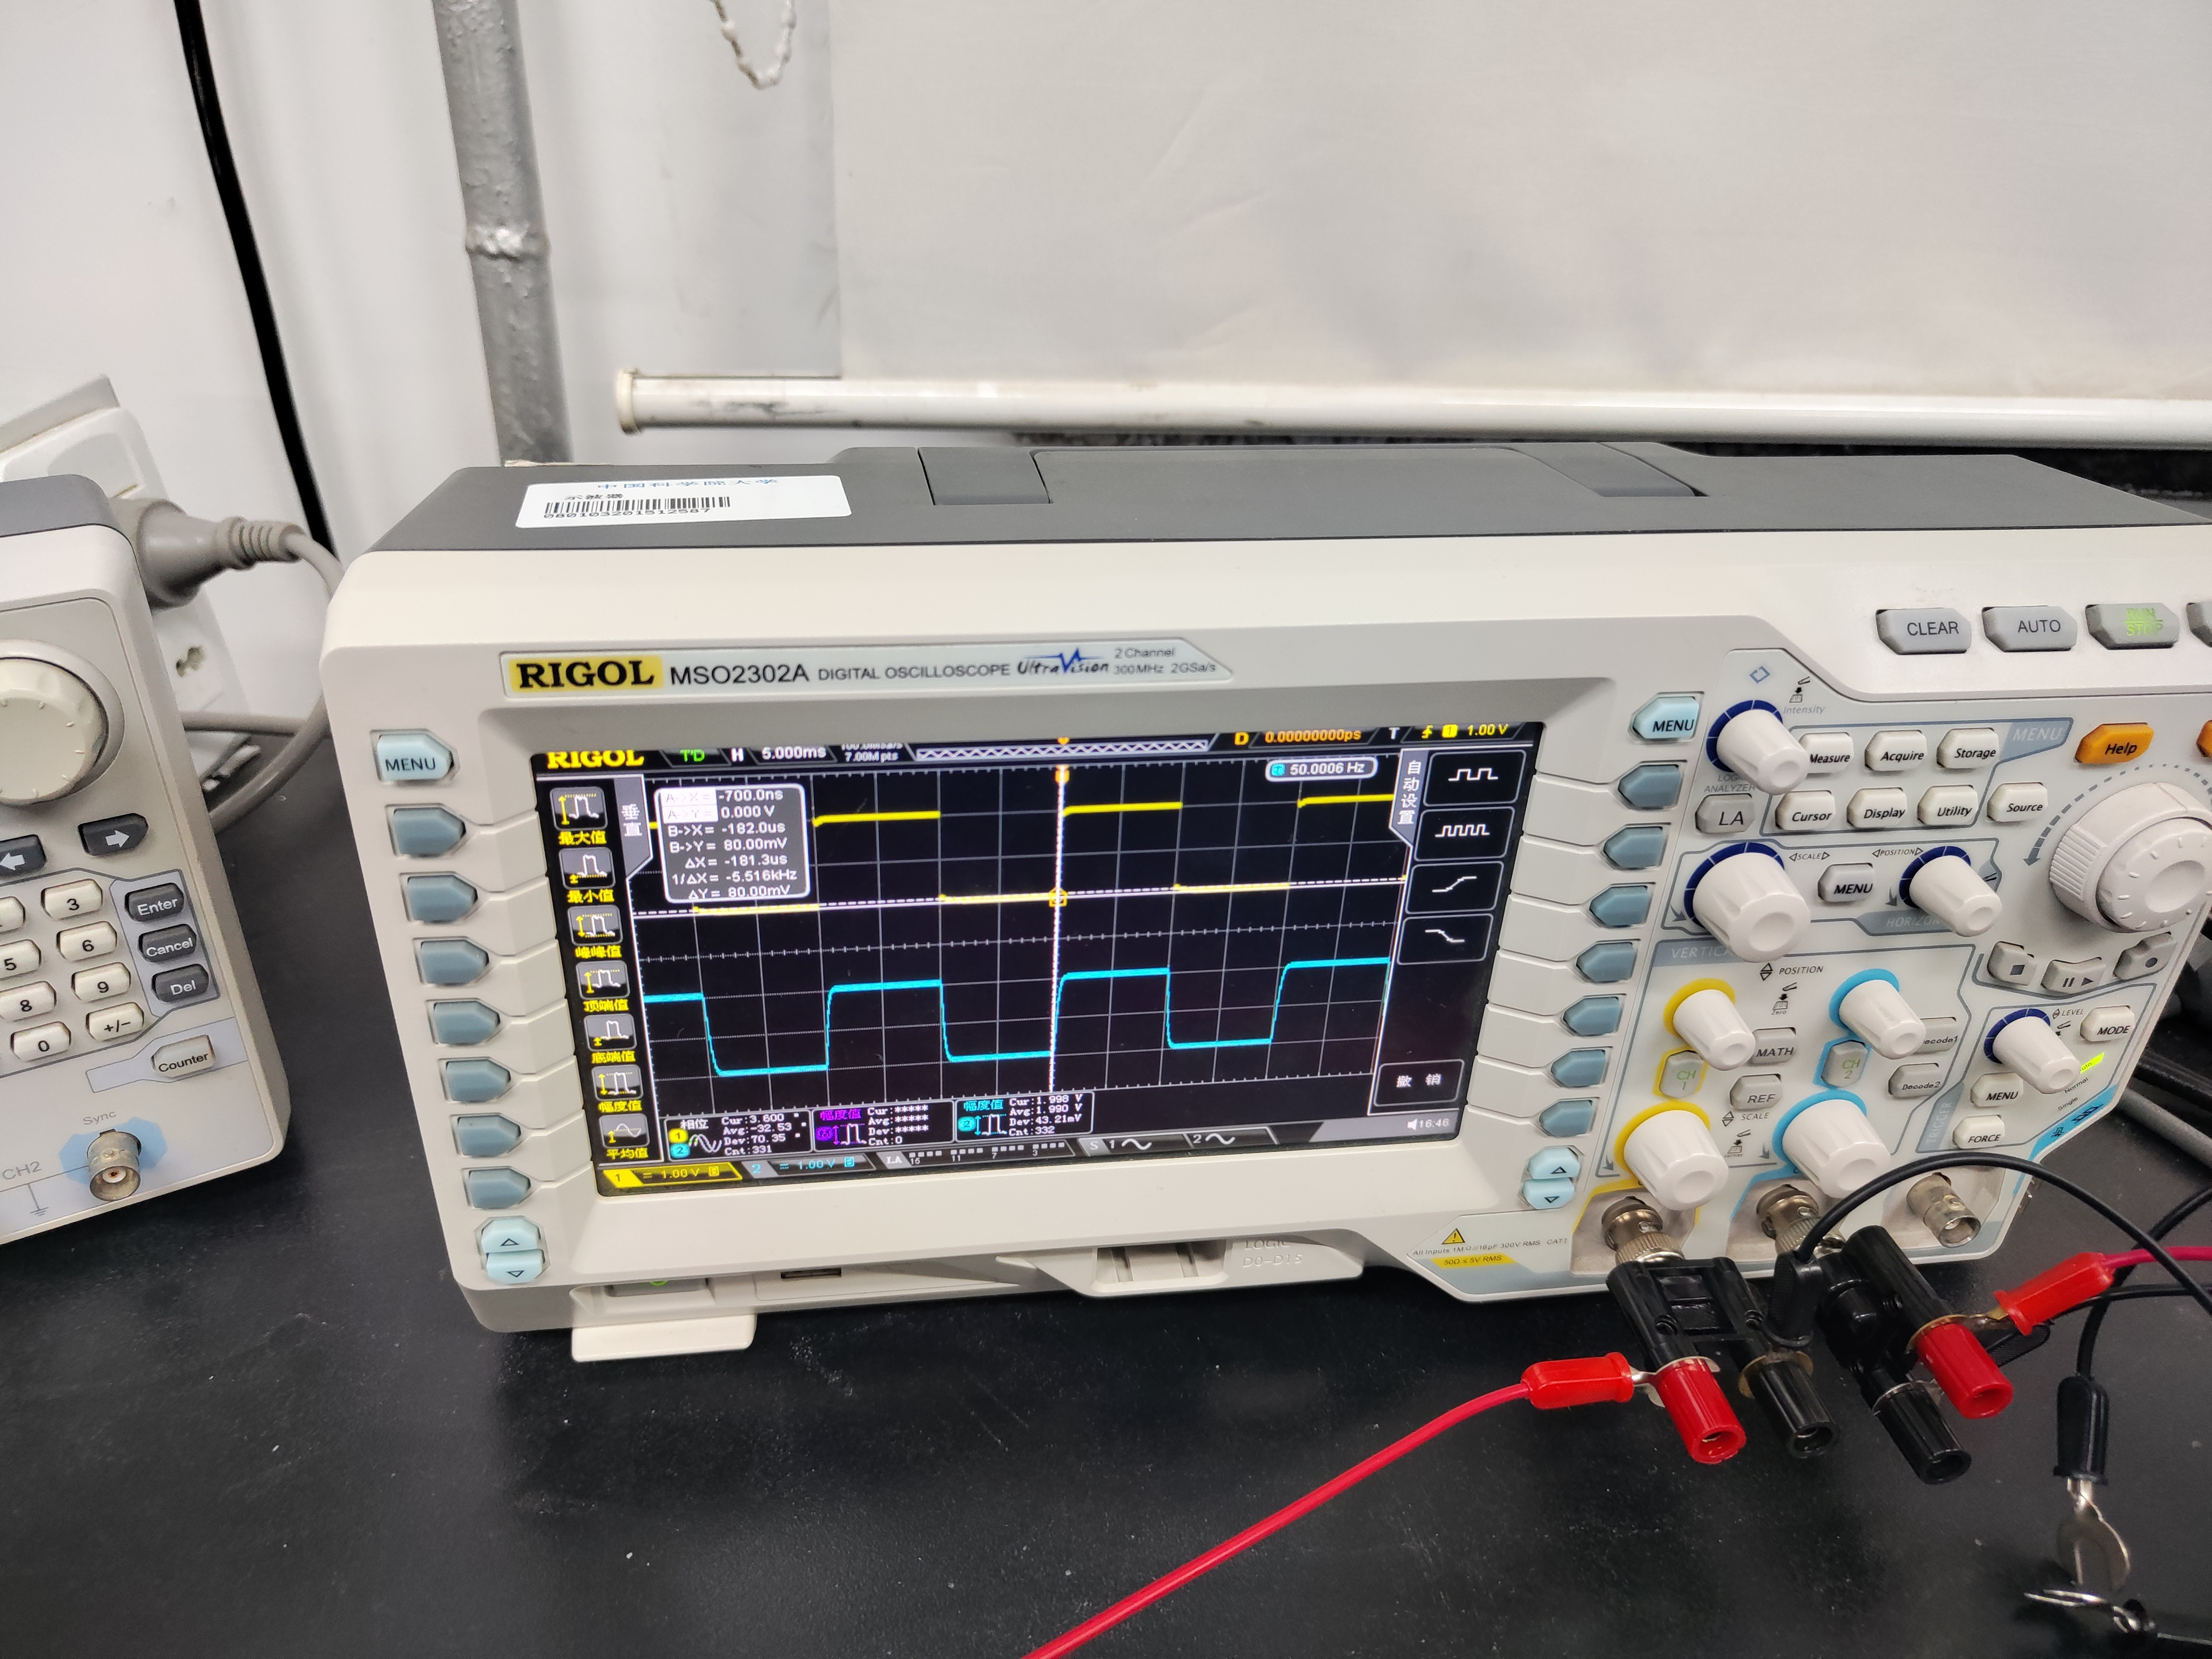
\includegraphics[width=5.5cm]{Fig/13.jpg}
                \caption{R=1400$\Omega$时暂态过程(其他同学设备)}
            \end{minipage}
        \end{figure}
        \hspace*{2em}在我的设备上,图15和图16无明显差别,难以区分。在其他同学设备上,$R=1400\Omega$时图像清晰。这可能和我的示波器探头倍数选择和阻抗设置有关。
        \newline \hspace*{2em}理论上,阻尼系数$\lambda=\frac{R}{2} \sqrt{\frac{C}{L}}=1$时为临界阻尼,此时$R_C=2\sqrt{\frac{L}{C}}=1414\Omega$。实际实验中,靠观察曲线差别确定临界阻尼过于困难。
    \end{enumerate}
    \item 第三组:$R=2k\Omega,f=250Hz$;第四组:$R=20k\Omega,f=20Hz$
    \begin{figure}[H]
        \begin{minipage}[t]{0.49\linewidth}
            \centering
            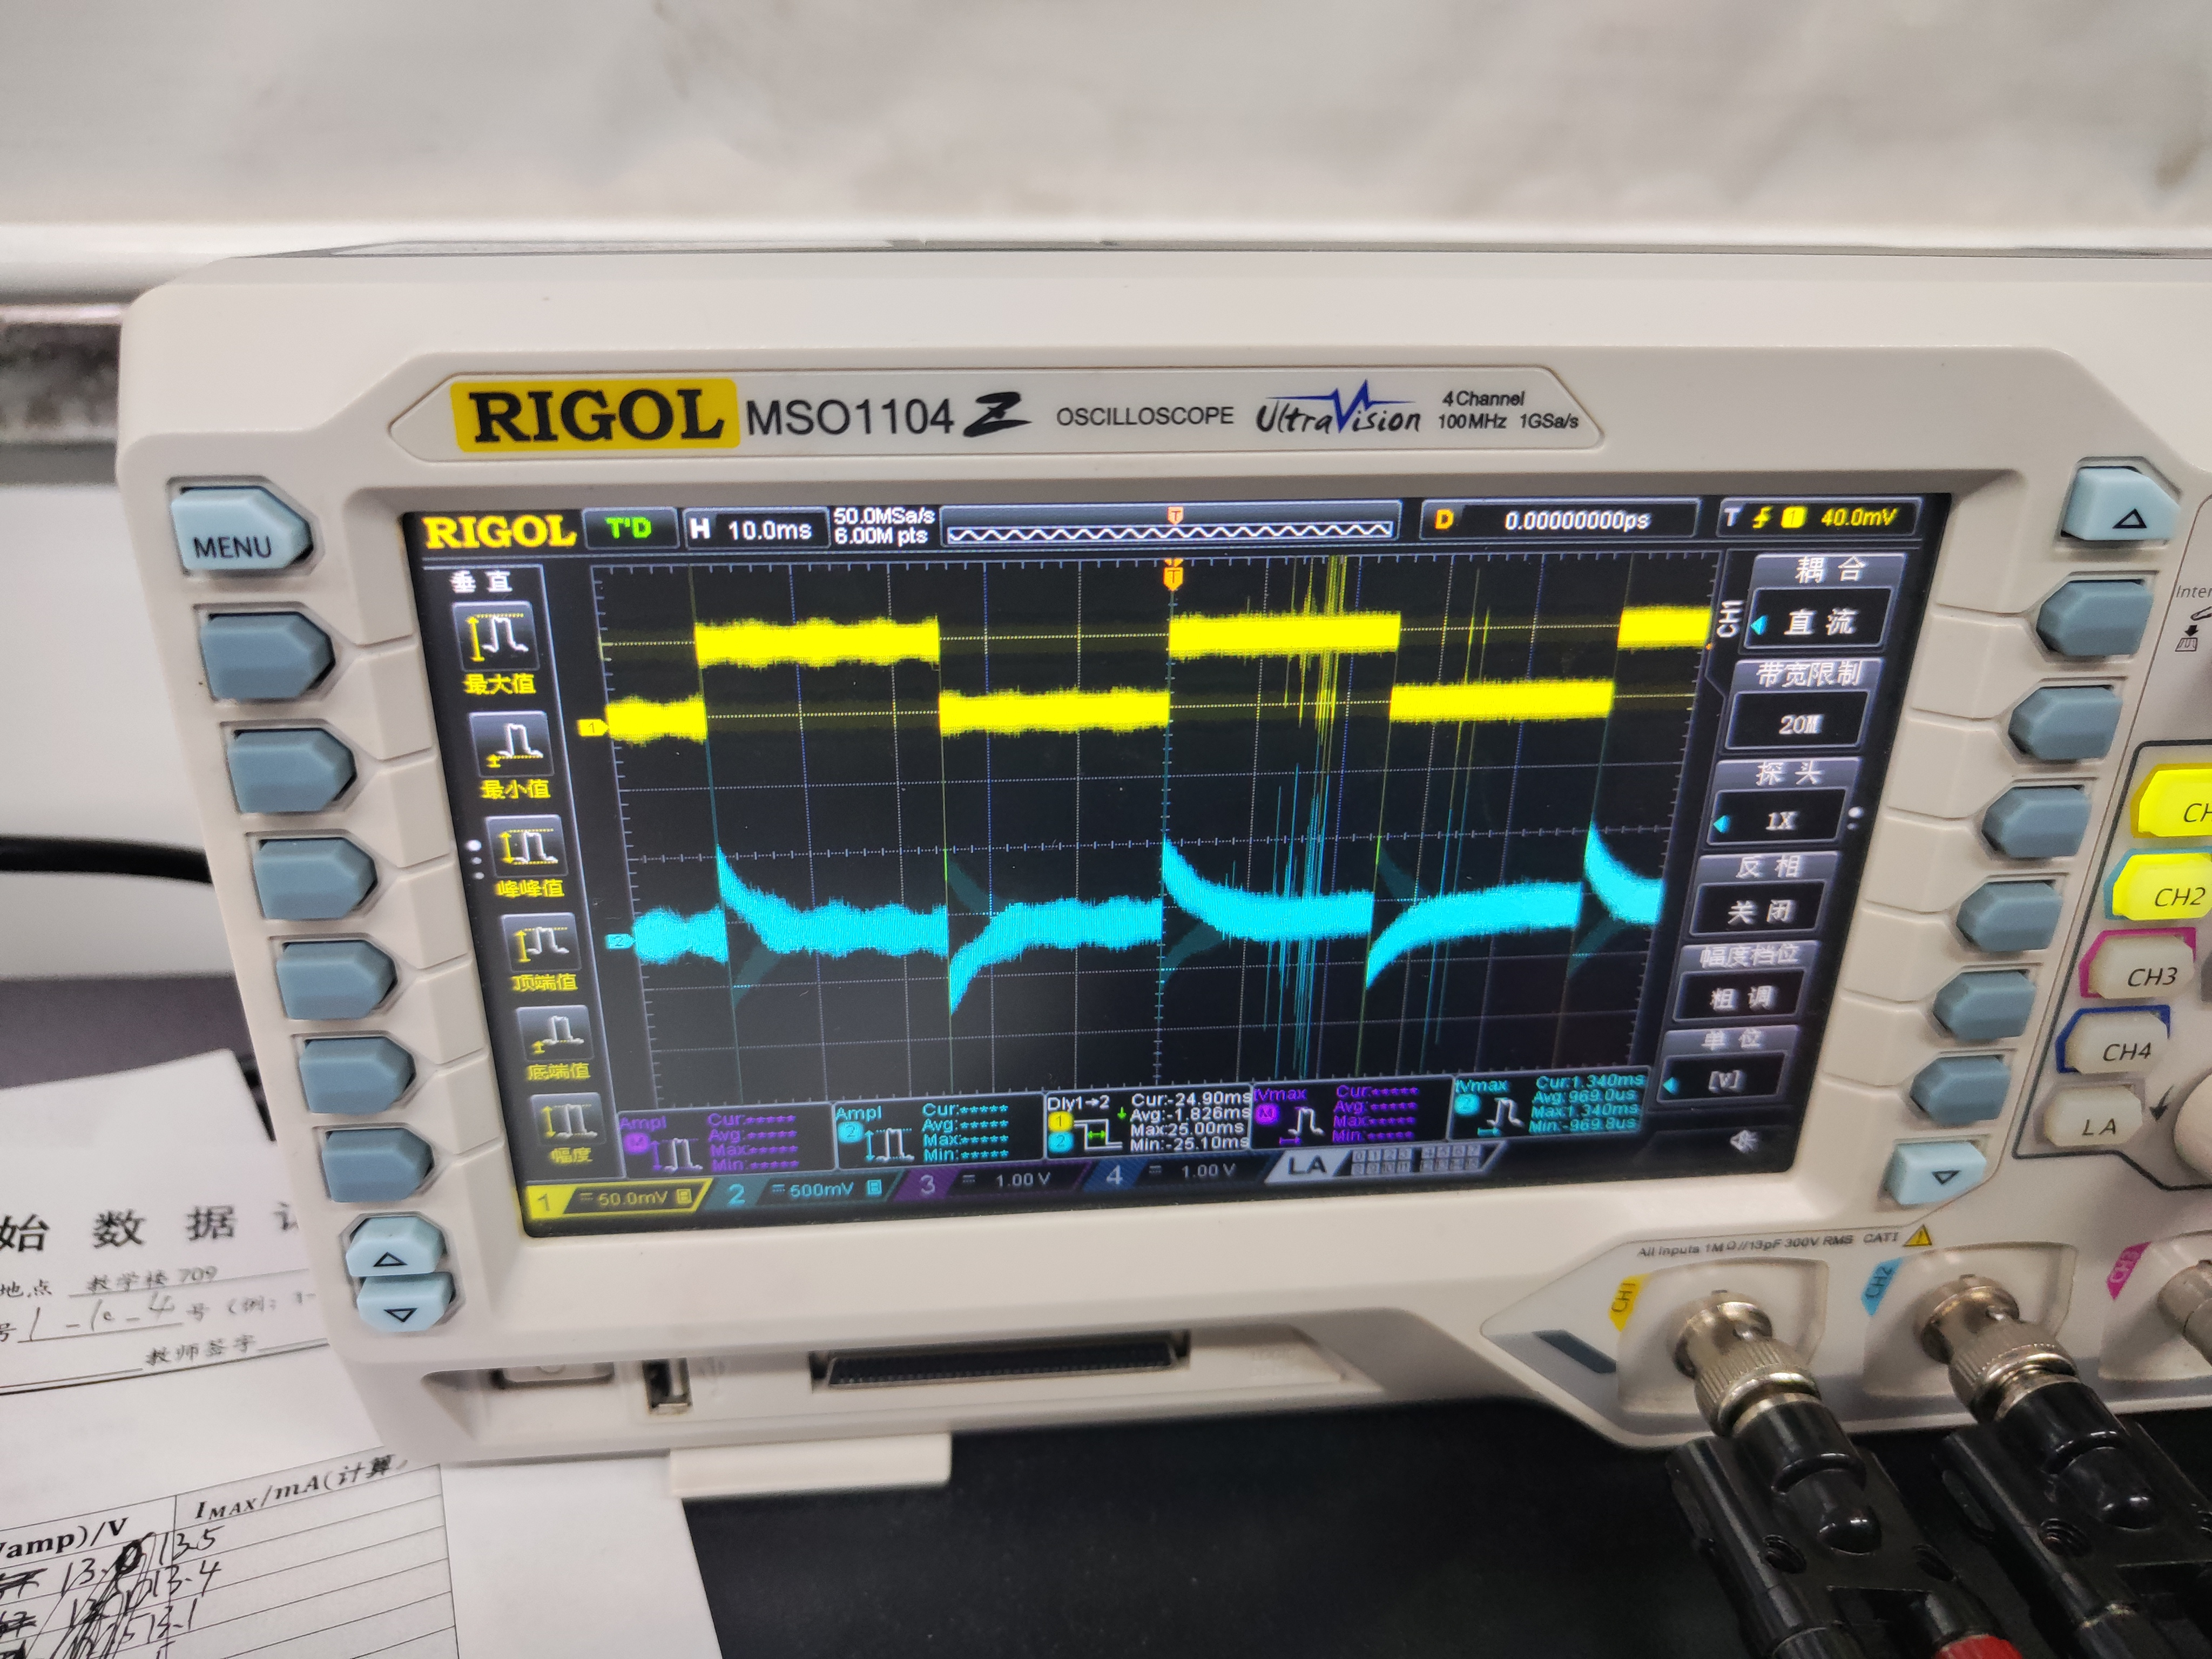
\includegraphics[width=6.5cm]{Fig/14.jpg}
            \caption{R=2k$\Omega$时暂态过程}
        \end{minipage}
        \begin{minipage}[t]{0.49\linewidth}
            \centering
            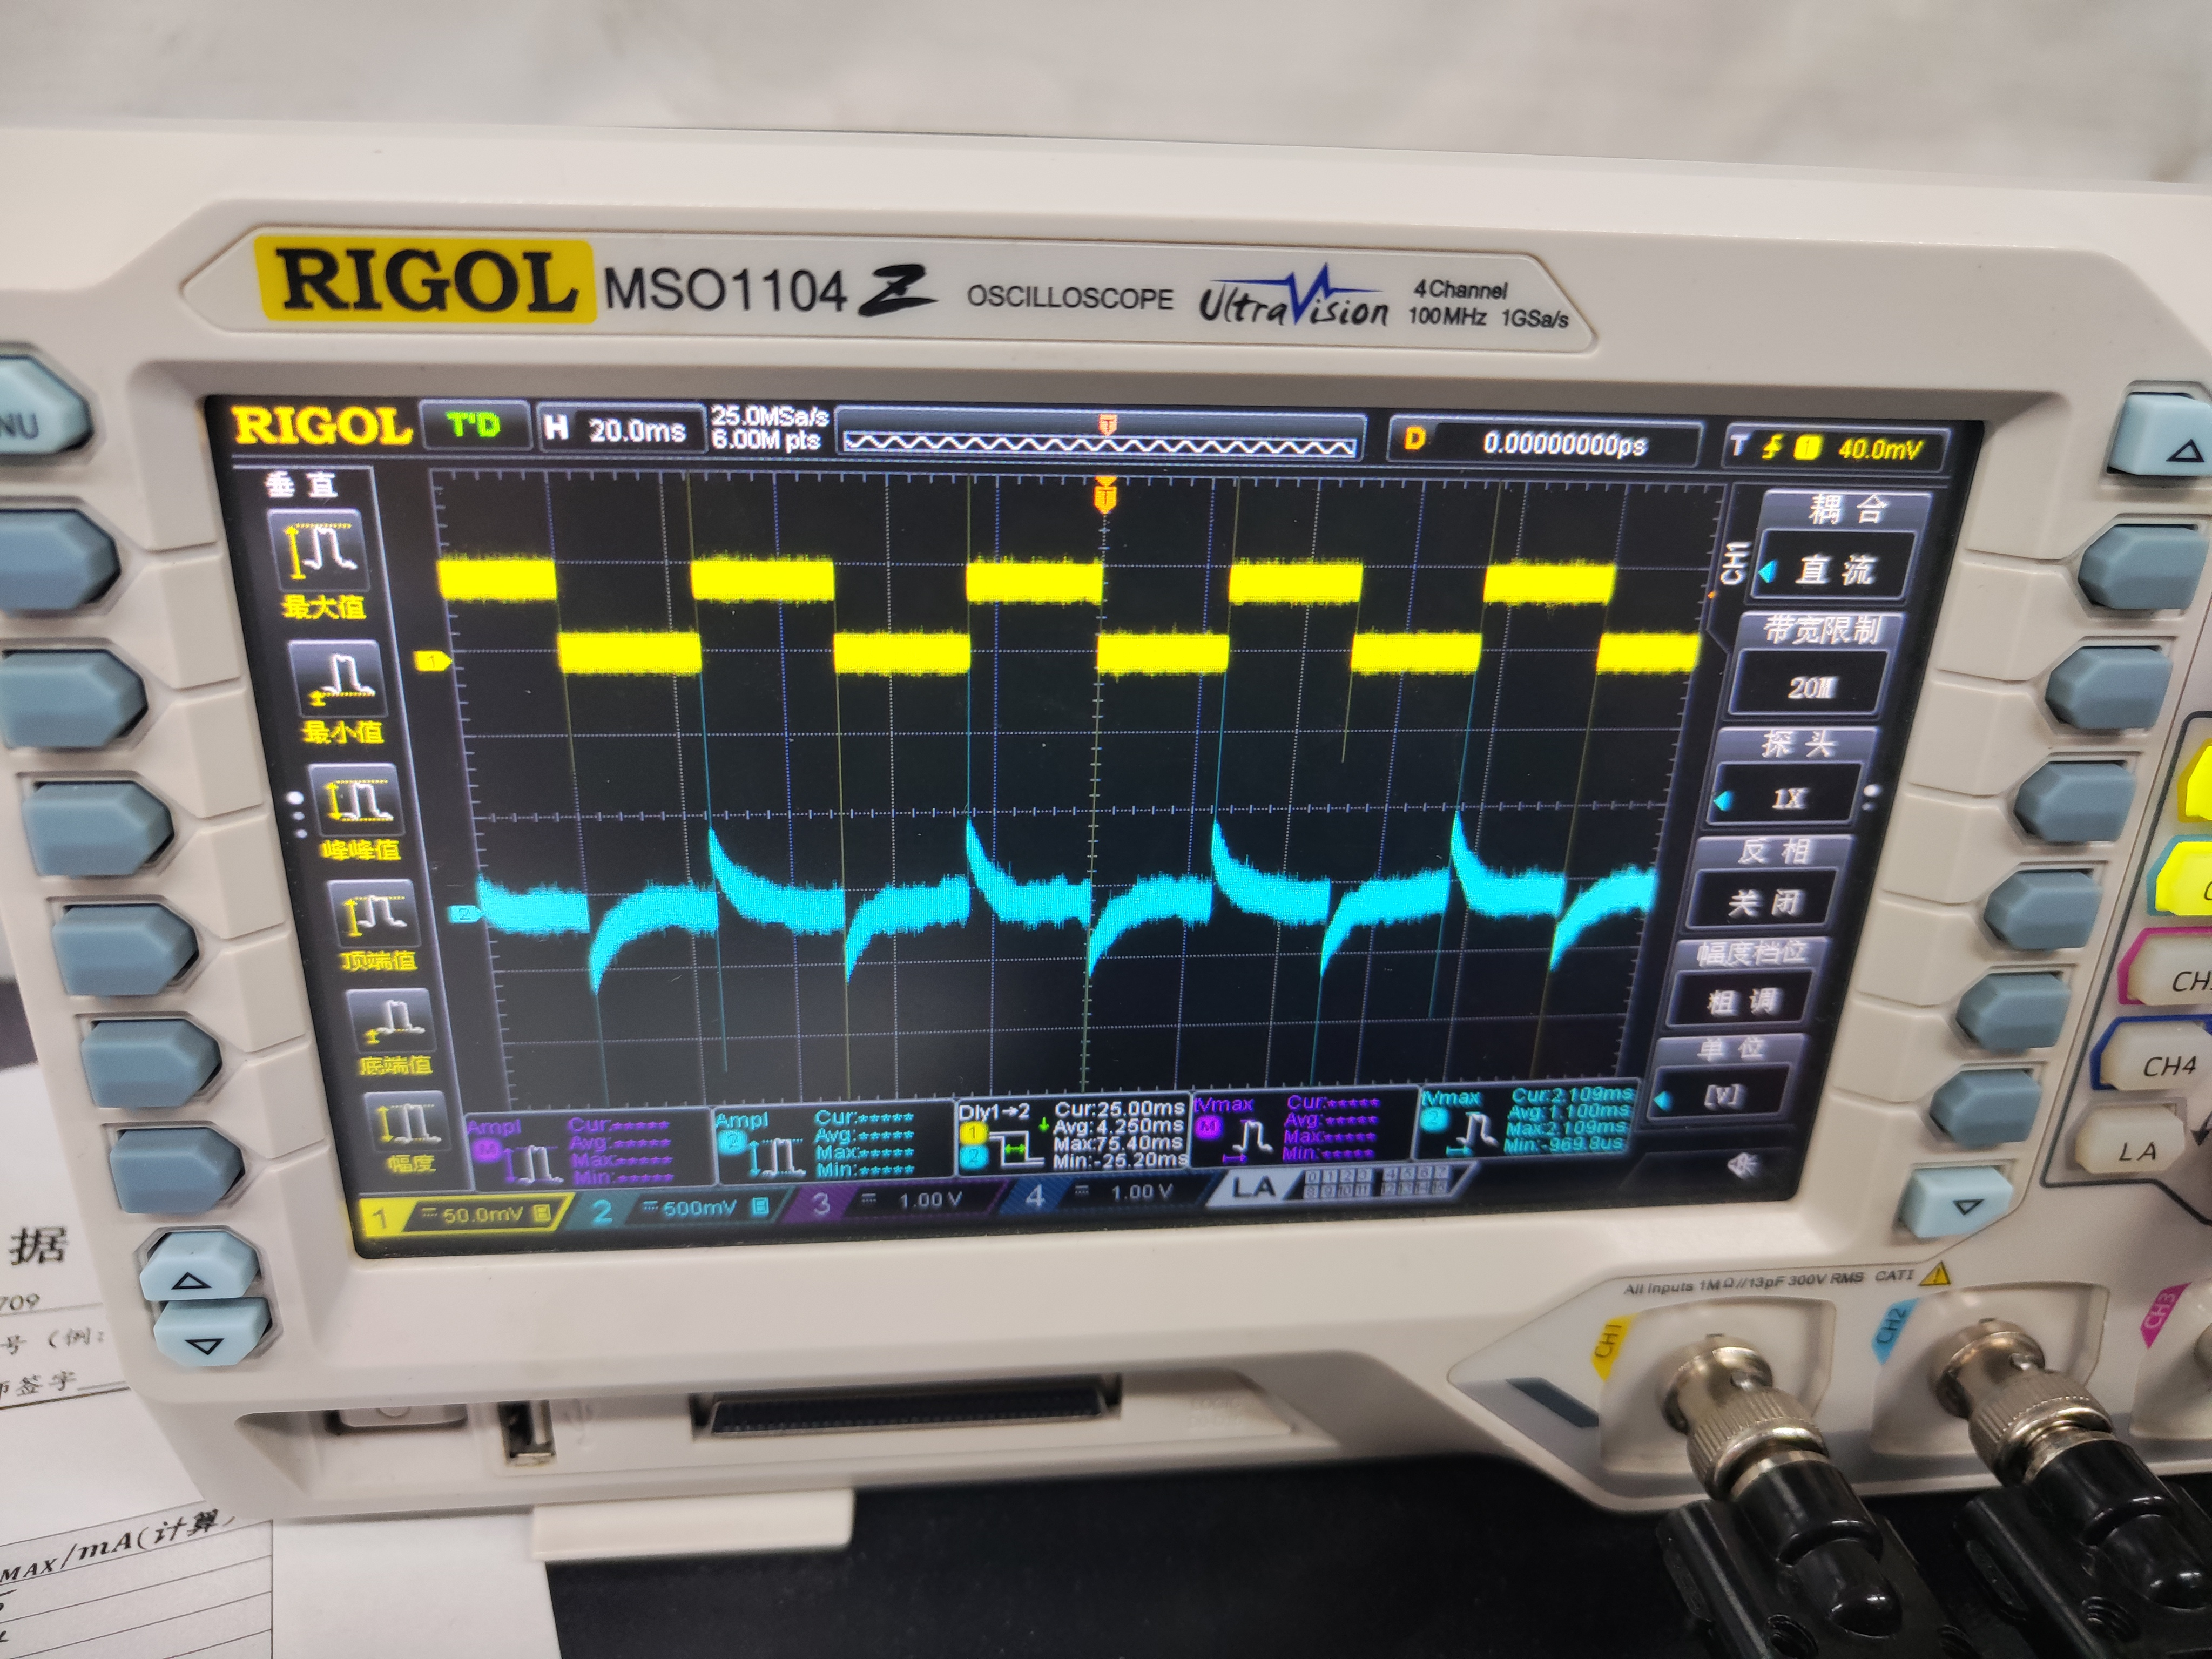
\includegraphics[width=6.5cm]{Fig/15.jpg}
            \caption{R=20k$\Omega$时暂态过程}
        \end{minipage}
    \end{figure}
    \hspace*{2em}由于条带过宽,难以观察。条带过宽的原因可能是示波器未正确调整,应使用交流耦合而非直流耦合。
\end{enumerate}
\section{实验反思、收获与总结}
\begin{enumerate}
    \item (最重要)使用示波器前,应该调整至适合实验测量范围的设置。本次实验基本使用默认设置,和实验需求差别很大,造成了一系列误差,如测量电压变成实际值的十倍需要手动调整的同时带来了巨大误差,观察暂态过程时图像过宽。要记住教训。
    \item 信号发生器输出波并不稳定,使用Avg功能测量能够减小误差。
    \item 关于实验顺序,应该先测$\varphi\text{-}i$的数据再寻找谐振频率。直接寻找谐振频率无异于大海捞针。本次实验我先寻找谐振频率,没有按照实验数据表上的推荐频率进行测试,浪费了一些时间。
    \item 本次实验中,我先是把信号发生器的红线接在电阻旁导致数据异常,后接在电容旁后正常。这告诉我们交流电仍旧有正负极之分,两线不一定等价。
    \item 关于测量相位差的方式有两种,一种是直接使用示波器输出相位差$\varphi$,另一种是取时间差$\Delta t$后计算相位差。时间差的精度更高,计算后更精确。直接测量相位差更加方便,在图像稳定时可采用。取时间差时可手动移动光标,也可用示波器时间差功能再取平均值。由于图像峰值较难精确手动接近,这两种做法区别不大,同样会产生误差。
    \item 共地操作在本实验的实验过程中没有特殊操作,示波器不同端口自动共地,并且几个电路元件在同一桌面上。没有未共地的反例,我暂时不知道共地与否除了安全上也许会造成短路意外还有什么其他区别。

\end{enumerate}

%空行
\bigskip
\begin{center}
    \vspace*{1em}
    \Large \bf 第二部分\qquad 实验原始记录
\end{center}
\includepdf[pages={1}]{Data/实验六 RLC谐振-数据记录表.pdf}

\end{document}